\chapter{Robustness analysis of outranking digraphs}
\label{sec:19}

\abstract*{ The required cardinal significance weights of the performance criteria represent the '\emph{Achilles}' heel of the outranking approach. Rarely will indeed a decision maker be cognitively competent for suggesting precise decimal-valued criteria significance weights. More often, the decision problem will involve more or less equally important decision objectives with more or less equi-significant criteria per objective. In this chapter, we study the robustness of the outranking digraph when the criteria significance weights faithfully indicate solely an order of importance.}

\abstract{ The required cardinal significance weights of the performance criteria represent the '\emph{Achilles}' heel of the outranking approach. Rarely will indeed a decision maker be cognitively competent for suggesting precise decimal-valued criteria significance weights. More often, the decision problem will involve more or less equally important decision objectives with more or less equi-significant criteria per objective. In this chapter, we study the robustness of the outranking digraph when the criteria significance weights faithfully indicate solely an order of importance.}

\section{Cardinal or ordinal criteria significance weights?}
\label{sec:19.1}

A random example of such a decision problem with equally important decision objectives and equi-significant criteria may be generated with the \texttt{Random3\-Objectives\-PerformanceTableau} class \index{Random3ObjectivesPerformanceTableau@\texttt{Random3ObjectivesPerformance\-Tableau()}}.

\begin{lstlisting}[caption={Generate a Random 3 Objectives Performance Tableau},label=list:19.1]
>>> from randomPerfTabs import \
...           Random3ObjectivesPerformanceTableau
>>> pt = Random3ObjectivesPerformanceTableau(\
...           numberOfActions=7,\
...           numberOfCriteria=9,seed=102)
>>> pt
    *------- PerformanceTableau instance description ------*
    Instance class   : Random3ObjectivesPerformanceTableau
    Seed             : 102
    Instance name    : random3ObjectivesPerfTab
    Actions          : 7
    Objectives       : 3
    Criteria         : 9
    NA proportion (%): 0.0
    Attributes       : ['name', 'valueDigits', 'BigData',
              'OrdinalScales', 'missingDataProbability',
              'negativeWeightProbability', 'randomSeed',
              'sumWeights', 'valuationPrecision',
              'commonScale', 'objectiveSupportingTypes',
              'actions', 'objectives', 'criteriaWeightMode',
              'criteria', 'evaluation', 'weightPreorder']
>>> pt.showObjectives()
  *------ show objectives -------*
   Eco: Economical aspect
     ec1 criterion of objective Eco 8
     ec4 criterion of objective Eco 8
     ec8 criterion of objective Eco 8
     Total weight: 24.00 (3 criteria)
   Soc: Societal aspect
     so2 criterion of objective Soc 12
     so7 criterion of objective Soc 12
     Total weight: 24.00 (2 criteria)
   Env: Environmental aspect
     en3 criterion of objective Env 6
     en5 criterion of objective Env 6
     en6 criterion of objective Env 6
     en9 criterion of objective Env 6
     Total weight: 24.00 (4 criteria)
\end{lstlisting}

In Listing~\ref{list:19.1} above one may notice a performance tableau \texttt{pt} describing seven decision alternatives that are assessed with respect to three equally important decision objectives concerning:
\begin{enumerate}[topsep=1pt]
\item An \emph{economical} aspect with a coalition of three performance criteria of significance weight 8 (Line 24),
\item A \emph{societal} aspect with a coalition of two performance criteria of significance weight 12 (Line 29), and
\item An \emph{environmental} aspect with a coalition of four performance criteria of significance weight 6 (Line 33).
\end{enumerate}

The question we tackle in this chapter is the following: How \emph{dependent} on the actual values of the significance weights appears to be the corresponding bipolar-valued outranking digraph? In the previous Chapter~\ref{sec:18} we assumed that the criteria significance weights were random variables. Here, we shall assume that we know for sure only the preordering of the significance weights.

In the random performance tableau \texttt{pt} we observe three increasing weight equivalence classes.
\begin{lstlisting}[caption={The significance weights preorder},label=list:19.2]
>>> pt.showWeightPreorder()
    ['en3', 'en5', 'en6', 'en9'] (6) <
    ['ec1', 'ec4', 'ec8'] (8) <
    ['so2', 'so7'] (12)
\end{lstlisting}

How robust will appear now the validated outranking and outranked situations when allowing all possible significance weights that are compatible with the weights preorder shown above \citep*{BIS-2009,BIS-2014Robust}?

\section{Qualifying the stability of outranking situations}
\label{sec:19.2}

Let us construct the bipolar-valued outranking digraph corresponding to the random 3-Objectives performance tableau \texttt{pt}.
\begin{lstlisting}[caption={Example Bipolar Outranking Digraph},label=list:19.3]
>>> from outrankingDigraphs import BipolarOutrankingDigraph
>>> g = BipolarOutrankingDigraph(pt)
>>> g.showRelationTable()
  * ---- Relation Table -----
   r(>=) |  'p1'   'p2'   'p3'   'p4'   'p5'   'p6'   'p7'   
   ------|------------------------------------------------
    'p1' | +1.00  -0.42  +0.00  -0.69  +0.39  +0.11  -0.06  
    'p2' | +0.58  +1.00  +0.83  +0.00  +0.58  +0.58  +0.58  
    'p3' | +0.25  -0.33  +1.00  +0.00  +0.50  +1.00  +0.25  
    'p4' | +0.78  +0.00  +0.61  +1.00  +1.00  +1.00  +0.67  
    'p5' | -0.11  -0.50  -0.25  -0.89  +1.00  +0.11  -0.14  
    'p6' | +0.22  -0.42  +0.00  -1.00  +0.17  +1.00  -0.11  
    'p7' | +0.22  -0.50  +0.17  -0.06  +0.78  +0.42  +1.00  
\end{lstlisting}

In Listing~\vref{list:19.3} Lines 7-13, we notice on the principal diagonal of the relation table the certainly validated reflexive terms $+1.00$; they are trivially independent of any significance weights. Now, we know for sure that \emph{unanimous} outranking situations are also completely independent of the significance weights. And, all outranking situations that are supported by a majority significance in each coalition of equi-significant criteria are as well independent of the actual importance we attach to each individual criteria coalition. We are furthermore able to effectively test if an outranking situation remains valid with all potential significance weights that are compatible with the given preordering shown in Listing~\vref{list:19.2} \citep{BIS-2014}. Mind that usually one obtains more or less numerous outranking situations that are in fact \emph{dependent} on the precise cardinal significance weights given to the criteria.

Such a \emph{stability denotation}\index{stability denotation} of outranking situations can be inspected using the \texttt{StabilityDenotation=True} flag \index{StabilityDenotation@\texttt{StabilityDenotation} flag} with the \texttt{showRelation\-Table()} method.
\begin{lstlisting}[caption={Bipolar-valued outranking relation table with stability denotation},label=list:19.4]
>>> g.showRelationTable(StabilityDenotation=True)
  * ---- Relation Table -----
   r/(stab)  |  'p1'  'p2'  'p3'  'p4'  'p5'  'p6'  'p7'   
   ----------|------------------------------------------
     'p1'    | +1.00 -0.42 +0.00 -0.69 +0.39 +0.11 -0.06  
             |  (+4)  (-2)  (+0)  (-3)  (+2)  (+2)  (-1)  
     'p2'    | +0.58 +1.00 +0.83  0.00 +0.58 +0.58 +0.58  
             |  (+2)  (+4)  (+3)  (+2)  (+2)  (+2)  (+2)  
     'p3'    | +0.25 -0.33 +1.00  0.00 +0.50 +1.00 +0.25  
             |  (+2)  (-2)  (+4)   (0)  (+2)  (+2)  (+1)  
     'p4'    | +0.78  0.00 +0.61 +1.00 +1.00 +1.00 +0.67  
             |  (+3)  (-1)  (+3)  (+4)  (+4)  (+4)  (+2)  
     'p5'    | -0.11 -0.50 -0.25 -0.89 +1.00 +0.11 -0.14  
             |  (-2)  (-2)  (-2)  (-3)  (+4)  (+2)  (-2)  
     'p6'    | +0.22 -0.42  0.00 -1.00 +0.17 +1.00 -0.11
             |  (+2)  (-2)  (+1)  (-2)  (+2)  (+4)  (-2)  
     'p7'    | +0.22 -0.50 +0.17 -0.06 +0.78 +0.42 +1.00  
             |  (+2)  (-2)  (+1)  (-1)  (+3)  (+2)  (+4)  
\end{lstlisting}

In Listing~\ref{list:19.4} above we may hence distinguish the following bipolar-valued stability levels:
\begin{itemize}[leftmargin=1cm]
\item [$\mathbf{\pm 4}$:] \emph{unanimous} outranking, resp. outranked, situation. The pairwise trivial reflexive outrankings, for instance, all show this stability level;
\item [$\mathbf{\pm 3}$:] validated outranking, resp. outranked, situation in \emph{each} coalition of equi-significant criteria. This is, for instance, the case for the outranking situation observed between alternatives \texttt{p1} and \texttt{p4} (see Lines 6 and 12);
\item [$\mathbf{\pm 2}$:] validated outranking, resp. outranked situation with \emph{all} potential significance weights that are \emph{compatible} With the given significance preorder (see List.~\vref{list:19.2}). This is the case when comparing alternatives \texttt{p1} and \texttt{p2} (see Lines 6 and 8);
\item [$\mathbf{\pm 1}$:] validated outranking, resp. outranked situation with the \emph{precisely given decimal} significance weights, a situation we may observe between alternatives \texttt{p3} and \texttt{p7} (see Lines 10 and 16);
\item [$\mathbf{0}$:] \texttt{indeterminate} outranking situation, like the one between alternatives \texttt{p1} and \texttt{p3} (see Lines 6 and 10).
\end{itemize}

It is worthwhile noticing that, in the one limit case where all performance criteria appear equi-significant --there is given a single equivalence class containing all the criteria significance weights-- one may only distinguish stability levels $\pm 4$ and $\pm 3$. In the other limit case, when all performance criteria admit different significance weights, the significance weights may be linearly ordered without ties and no stability level $\pm 3$ can be observed.

As mentioned above, all reflexive comparisons trivially confirm an unanimous outranking situation: all decision alternatives are indeed always``\emph{at least as well evaluated as}'' themselves. But there appear also two non reflexive unanimous outranking situations: when comparing, for instance, alternative \texttt{p4} with alternatives \texttt{p5} and \texttt{p6} (see List.~\vref{list:19.4} Lines 14 and 16). Let us inspect the details of how alternatives \texttt{p4} and \texttt{p5} compare.
\begin{lstlisting}
>>> g.showPairwiseComparison('p4','p5')
 *------------  pairwise comparison ----*
  Comparing actions : (p4, p5)
  crit. wght.  g(x)  g(y)    diff  | ind   pref    r()
  ec1   8.00  85.19  46.75  +38.44 | 5.00  10.00   +8.00
  ec4   8.00  72.26   8.96  +63.30 | 5.00  10.00   +8.00
  ec8   8.00  44.62  35.91   +8.71 | 5.00  10.00   +8.00
  en3   6.00  80.81  31.05  +49.76 | 5.00  10.00   +6.00
  en5   6.00  49.69  29.52  +20.17 | 5.00  10.00   +6.00
  en6   6.00  66.21  31.22  +34.99 | 5.00  10.00   +6.00
  en9   6.00  50.92   9.83  +41.09 | 5.00  10.00   +6.00
  so2  12.00  49.05  12.36  +36.69 | 5.00  10.00  +12.00
  so7  12.00  55.57  44.92  +10.65 | 5.00  10.00  +12.00
  Valuation in range: -72.00 to +72.00;          -------
                             global concordance:  +72.00
\end{lstlisting}

Alternative \texttt{p4} is indeed  unanimously ``\emph{at least as well evaluated as}'' alternative \texttt{p5} and $r(p4 \succsim p5)\; =\; 72/72\; =\; +1.00$ (see List.~\vref{list:19.4} Line 11). The converse comparison does not, however, reveal such an unanimous outranked situation. 
\begin{lstlisting}
>>> g.showPairwiseComparison('p5','p4')
 *------------  pairwise comparison ----*
  Comparing actions : (p5, p4)
  crit. wght.  g(x)  g(y)    diff  | ind   pref     r()
  ec1   8.00  46.75  85.19  -38.44 | 5.00  10.00   -8.00
  ec4   8.00   8.96  72.26  -63.30 | 5.00  10.00   -8.00
  ec8   8.00  35.91  44.62   -8.71 | 5.00  10.00   +0.00
  en3   6.00  31.05  80.81  -49.76 | 5.00  10.00   -6.00
  en5   6.00  29.52  49.69  -20.17 | 5.00  10.00   -6.00
  en6   6.00  31.22  66.21  -34.99 | 5.00  10.00   -6.00
  en9   6.00   9.83  50.92  -41.09 | 5.00  10.00   -6.00
  so2  12.00  12.36  49.05  -36.69 | 5.00  10.00  -12.00
  so7  12.00  44.92  55.57  -10.65 | 5.00  10.00  -12.00
  Valuation in range: -72.00 to +72.00;           ------
                             global concordance:  -64.00
\end{lstlisting}

The converse comparison only qualifies at stability level $-3$ (see List.~\vref{list:19.4} Line 13); $r(p5 \succsim p4)\; =\; -64/72\; =\; -0.89$). On criterion \texttt{ec8} we observe in fact a small negative performance difference of $-8.71$ (see Line 7 above) which is effectively below the supposed preference discrimination threshold of $10.00$. Yet, the outranked situation is supported by a majority of criteria in each decision objective. Hence, the reported preferential situation is completely independent of any chosen significance weights.

Let us now consider a comparison, like the one between alternatives \texttt{p2} and \texttt{p1}, that is qualified at stability level $+2$, resp. $-2$.
\begin{lstlisting}[caption={Comparison of alternatives \texttt{p2} and \texttt{p1}},label=list:19.5]
>>> g.showPairwiseOutrankings('p2','p1')
  *------------  pairwise comparison ----*
   Comparing actions : (p2, p1)
   crit. wght.  g(x)  g(y)    diff  | ind   pref     r()
   ec1   8.00  89.77  38.11  +51.66 | 5.00  10.00   +8.00
   ec4   8.00  86.00  22.65  +63.35 | 5.00  10.00   +8.00
   ec8   8.00  89.43  77.02  +12.41 | 5.00  10.00   +8.00
   en3   6.00  20.79  58.16  -37.37 | 5.00  10.00   -6.00
   en5   6.00  23.83  31.40   -7.57 | 5.00  10.00   +0.00
   en6   6.00  18.66  11.41   +7.25 | 5.00  10.00   +6.00
   en9   6.00  26.65  44.37  -17.72 | 5.00  10.00   -6.00
   so2  12.00  89.12  22.43  +66.69 | 5.00  10.00  +12.00
   so7  12.00  84.73  28.41  +56.32 | 5.00  10.00  +12.00
   Valuation in range: -72.00 to +72.00;          -------
                              global concordance:  +42.00
    *------------  pairwise comparison ----*
    Comparing actions : ('p1', 'p2')
    crit. wght.  g(x)  g(y)    diff  | ind   pref     r()
    ec1   8.00  38.11  89.77  -51.66 | 5.00  10.00   -8.00
    ec4   8.00  22.65  86.00  -63.35 | 5.00  10.00   -8.00
    ec8   8.00  77.02  89.43  -12.41 | 5.00  10.00   -8.00
    en3   6.00  58.16  20.79  +37.37 | 5.00  10.00   +6.00
    en5   6.00  31.40  23.83   +7.57 | 5.00  10.00   +6.00 
    en6   6.00  11.41  18.66   -7.25 | 5.00  10.00   +0.00
    en9   6.00  44.37  26.65  +17.72 | 5.00  10.00   +6.00
    so2  12.00  22.43  89.12  -66.69 | 5.00  10.00  -12.00
    so7  12.00  28.41  84.73  -56.32 | 5.00  10.00  -12.00
    Valuation in range: -72.00 to +72.00;          -------
                                global concordance: -30.00
\end{lstlisting}

In both comparisons, the evaluations observed with respect to the environmental decision objective are not validating with a significant majority the outranking, resp. outranked, situation. Hence, the stability of the reported preferential situations is in fact dependent on choosing significance weights that are compatible with the given significance weights preorder (see List.~\vref{list:19.2}).

Let us finally inspect a comparison that is only qualified at stability level $+1$, like the one between alternatives \texttt{p7} and \texttt{p3}.
\begin{lstlisting}[caption={Comparison of alternatives \texttt{p7} and \texttt{p3}},label=list:19.6]
>>> g.showPairwiseOutrankings('p7','p3')
 *------------  pairwise comparison ----*
  Comparing actions : ('p7', 'p3')
  crit. wght.  g(x)  g(y)    diff  | ind   pref     r()
  ec1   8.00  15.33  80.19  -64.86 | 5.00  10.00   -8.00
  ec4   8.00  36.31  68.70  -32.39 | 5.00  10.00   -8.00
  ec8   8.00  38.31  91.94  -53.63 | 5.00  10.00   -8.00
  en3   6.00  30.70  46.78  -16.08 | 5.00  10.00   -6.00
  en5   6.00  35.52  27.25   +8.27 | 5.00  10.00   +6.00
  en6   6.00  69.71   1.65  +68.06 | 5.00  10.00   +6.00
  en9   6.00  13.10  14.85   -1.75 | 5.00  10.00   +6.00
  so2  12.00  68.06  58.85   +9.21 | 5.00  10.00  +12.00
  so7  12.00  58.45  15.49  +42.96 | 5.00  10.00  +12.00
  Valuation in range: -72.00 to +72.00;          -------
                              global concordance: +12.00
 *------------  pairwise comparison ----*
  Comparing actions : ('p3', 'p7')
  crit. wght.  g(x)  g(y)    diff  | ind   pref     r()
  ec1   8.00  80.19  15.33  +64.86 | 5.00  10.00   +8.00
  ec4   8.00  68.70  36.31  +32.39 | 5.00  10.00   +8.00
  ec8   8.00  91.94  38.31  +53.63 | 5.00  10.00   +8.00
  en3   6.00  46.78  30.70  +16.08 | 5.00  10.00   +6.00
  en5   6.00  27.25  35.52   -8.27 | 5.00  10.00   +0.00
  en6   6.00   1.65  69.71  -68.06 | 5.00  10.00   -6.00
  en9   6.00  14.85  13.10   +1.75 | 5.00  10.00   +6.00
  so2  12.00  58.85  68.06   -9.21 | 5.00  10.00   +0.00
  so7  12.00  15.49  58.45  -42.96 | 5.00  10.00  -12.00
  Valuation in range: -72.00 to +72.00;          -------
                              global concordance: +18.00
\end{lstlisting}

In both cases, choosing only significances that are compatible with the given weights preorder will not always result in positively validated outranking situations.

\section{Computing the stability denotation of outranking situations}
\label{sec:19.3}

Stability levels $\pm 4$ and $\pm 3$ are, the case given, easy to detect. Detecting a stability level $\pm 2$ is far less obvious.  Now, it is precisely again the bipolar-valued epistemic characteristic domain that will give us a way to implement an effective test for stability level $+2$ and $-2$ \citep{BIS-2004b,BIS-2004c}. 

Let us consider the significance equivalence classes we observe in the given weights preorder. Here we observe three weight classes: $6$, $8$, and $12$, in increasing order (see List.~\vref{list:19.2}). In the pairwise comparisons, shown above, these equivalence classes may appear positively or negatively, besides the indeterminate significance of value $0.00$. We thus get the following ordered bipolar list of significance weights: $W = [-12, -8, -6, 0, 6, 8, 12]$.

In all the pairwise marginal comparisons shown in the previous Section, we may observe that each one of the nine criteria assigns one precise item out of this list $W$. Let us denote $q[i]$ the number of criteria assigning item $W[i]$, and $Q[i]$ the cumulative sums of these $q[i]$ counts, where $i$ is an index in the range of the length of list $W$.

In the comparison of alternatives \texttt{p2} and \texttt{p1}, for instance (see List.~\vref{list:19.5}), we observe the following counts: \hfill
\begin{center}
\begin{tabular}{l|r|r|r|r|r|r|r}
 \svhline\noalign{\smallskip}
  $W[i]$ & -12 & -8  & -6  &  0  &  6  &  8 &  12\\  
 \noalign{\smallskip}\hline\noalign{\smallskip}
$q[i]$  &  0 &  0 &   2 &   1  &  1  &  3  &  2 \\
$Q[i]$  &  0 &  0 &   2 &   3  &  4  &  7  &  9 \\
      \noalign{\smallskip}\hline
\end{tabular}
\end{center}

Let use denote $-q$ and $-Q$ the reversed versions of the $q$ and the $Q$ lists. We thus obtain the following result.\hfill
\begin{center}
\begin{tabular}{l|r|r|r|r|r|r|r}
 \svhline\noalign{\smallskip}
  $W[i]$ & -12 & -8  & -6  &  0  &  6  &  8 &  12\\  
 \noalign{\smallskip}\hline\noalign{\smallskip}
  $-q[i]$  &  2 &  3 &   1 &   1  &  2  &  0  &  0 \\
  $-Q[i]$  &  2 &  5 &   6 &   7  &  9  &  9  &  9 \\
 \noalign{\smallskip}\hline
\end{tabular}
\end{center}

Now, a pairwise outranking situation will be qualified at stability level $+2$, i.e. positively validated with any significance weights that are compatible with the given weights preorder, when for all $i$, we observe $Q[i] \leq -Q[i]$ and there exists one $i$ such that $Q[i] < -Q[i]$. Similarly, a pairwise outranked situation will be qualified at stability level $-2$, when for all $i$, we observe $Q[i] \geq -Q[i]$ and there exists one $i$ such that $Q[i] > -Q[i]$ \citep{BIS-2004c}.

We may verify, for instance, that the outranking situation observed between alternatives \texttt{p2} and \texttt{p1} does indeed verify this \emph{first order distributional dominance} condition. \hfill
\begin{center}
\begin{tabular}{l|r|r|r|r|r|r|r}
 \svhline\noalign{\smallskip}
  $W[i]$ & -12 & -8  & -6  &  0  &  6  &  8 &  12\\  
 \noalign{\smallskip}\hline\noalign{\smallskip}
  $Q[i]$  &  0 &  0 &   2 &   3  &  4  &  7  &  9 \\
  $-Q[i]$  &  2 &  5 &   6 &   7  &  9  &  9  &  9 \\
 \noalign{\smallskip}\hline
\end{tabular}
\end{center}

Notice that outranking situations qualified at stability levels $\pm 4$ and $\pm 3$, evidently verify the stability level $\pm 2$ test above. The outranking situation between alternatives \texttt{p7} and \texttt{p3} does not, however, verify this test (see List.~\vref{list:19.6}).\hfill
\begin{center}
\begin{tabular}{l|r|r|r|r|r|r|r}
 \svhline\noalign{\smallskip}
  $W[i]$ & -12 & -8  & -6  &  0  &  6  &  8 &  12\\  
 \noalign{\smallskip}\hline\noalign{\smallskip}
  $q[i]$  &  0 &  3 &   1 &   0  &  3  &  0  &  2 \\
  $Q[i]$  &  0 &  3 &   4 &   4  &  7  &  7  &  9 \\
  $-Q[i]$  &  2 &  2 &   5 &   5  &  6  &  9  &  9 \\
 \noalign{\smallskip}\hline
\end{tabular}
\end{center}

This time, not all the $Q[i]$ are \emph{lower or equal} than the corresponding $-Q[i]$ terms. Hence the outranking situation between \texttt{p7} and \texttt{p3} is not positively validated with all potential significance weights that are compatible with the given weights preorder.

Using this stability denotation, we may, hence, define the following \emph{robust} version of a bipolar-valued outranking digraph.

\section{Robust bipolar-valued outranking digraphs}
\label{sec:19.4}

\begin{definition}[Robust outranking situation]\label{def:19.1}
\begin{itemize}
\item We say that decision alternative \texttt{x} \emph{robustly outranks} decision alternative \texttt{y} when:
\begin{itemize}[nosep]
\item \texttt{x} positively outranks \texttt{y} at stability level $+2$ or higher and
\item we may not observe any considerable counter-performance of \texttt{x} on a discordant criterion.
\end{itemize}
\item Dually, we say that decision alternative \texttt{x} \emph{does not robustly outrank} decision alternative \texttt{y} when:
\begin{itemize}[nosep]
\item \texttt{x} is positively outranked by \texttt{y} at stability level $-2$ or lower and
\item we may not observe any considerable better performance of \texttt{x} on a discordant criterion.
\end{itemize}
\item Otherwise the outranking situation is indeterminate.
\end{itemize}
\end{definition}

The corresponding \emph{robust} outranking digraph can be computed as follows with the \texttt{RobustOutrankingDigraph} class\index{RobustOutrankingDigraph@\texttt{RobustOutrankingDigraph} class}:
\begin{lstlisting}[caption={Computing a robust outranking digraph},label=list:19.7]
>>> from outrankingDigraphs import\
...              RobustOutrankingDigraph
>>> rg = RobustOutrankingDigraph(pt) # same pt
>>> rg
  *------- Object instance description ------*
   Instance class      : RobustOutrankingDigraph
   Instance name       : robust_random3ObjectivesPerfTab
   Actions             : 7
   Criteria            : 9
   Size                : 22
   Determinateness (%) : 68.45
   Valuation domain    : [-1.00;1.00]
   Attributes          : ['name', 'methodData', 'actions',
         'order', 'criteria', 'evaluation',
         'vetos', 'valuationdomain',
         'cardinalRelation', 'ordinalRelation',
         'equisignificantRelation', 'unanimousRelation',
         'relation', 'gamma', 'notGamma']
>>> rg.showRelationTable()
  * ---- Relation Table -----
   r/(stab) |  'p1'  'p2'  'p3'  'p4'  'p5'  'p6'  'p7'   
   ---------|------------------------------------------
     'p1'   | +1.00 -0.42 +0.00 -0.69 +0.39 +0.11 +0.00  
            |  (+4)  (-2)  (+0)  (-3)  (+2)  (+2)  (-1)  
     'p2'   | +0.58 +1.00 +0.83 +0.00 +0.58 +0.58 +0.58  
            |  (+2)  (+4)  (+3)  (+2)  (+2)  (+2)  (+2)  
     'p3'   | +0.25 -0.33 +1.00 +0.00 +0.50 +1.00 +0.00  
            |  (+2)  (-2)  (+4)  (+0)  (+2)  (+2)  (+1)  
     'p4'   | +0.78 +0.00 +0.61 +1.00 +1.00 +1.00 +0.67  
            |  (+3)  (-1)  (+3)  (+4)  (+4)  (+4)  (+2)  
     'p5'   | -0.11 -0.50 -0.25 -0.89 +1.00 +0.11 -0.14  
            |  (-2)  (-2)  (-2)  (-3)  (+4)  (+2)  (-2)  
     'p6'   | +0.22 -0.42 +0.00 -1.00 +0.17 +1.00 -0.11  
            |  (+2)  (-2)  (+1)  (-2)  (+2)  (+4)  (-2)  
     'p7'   | +0.22 -0.50 +0.00 +0.00 +0.78 +0.42 +1.00  
            |  (+2)  (-2)  (+1)  (-1)  (+3)  (+2)  (+4)  
\end{lstlisting}

All outranking situations, qualified at stability level $\pm 1$, are now put to an \emph{indeterminate} status (see List.~\ref{list:19.7} Lines 23-24 Column \texttt{p7}). In the example here, three positive outrankings get dropped: between \texttt{p3} and \texttt{p7}, between \texttt{p7} and \texttt{p3}, and between \texttt{p6} and \texttt{p3}, where the last situation is actually already doubtful because of a veto situation (see List.~\vref{list:19.7} Lines 22-35). Three negative outrankings get dropped as well: between \texttt{p1} and \texttt{p7}, between \texttt{p4} and \texttt{p2}, and between \texttt{p7} and \texttt{p4} (see Lines 22-35).

Notice by the way that outranking or outranked situations, although qualified at level $\pm 2$ or $\pm 3$ may nevertheless become doubtful because of considerable performance differences. We may observe such a doubtful situation when comparing, for instance, alternatives \texttt{p2} and \texttt{p4} (see List.~\vref{list:19.7} Lines 24-25).
\begin{lstlisting}[caption={Comparing alternatives \texttt{p2} and \texttt{p4}},label=list:19.8,basicstyle=\ttfamily\scriptsize]
>>> rg.showPairwiseComparison('p2','p4')
   *------------  pairwise comparison ----*
    Comparing actions : (p2, p4)
    crit. wght.  g(x)  g(y)    diff  	| ind   pref    r() 	|   v    veto
    -------------------------------------------------------------------------
    ec1   8.00  89.77  85.19  +4.58 	| 5.00  10.00   +8.00 	| 
    ec4   8.00  86.00  72.26  +13.74 	| 5.00  10.00   +8.00 	| 
    ec8   8.00  89.43  44.62  +44.81 	| 5.00  10.00   +8.00 	| 
    en3   6.00  20.79  80.81  -60.02 	| 5.00  10.00   -6.00 	| 60.00 -1.00
    en5   6.00  23.83  49.69  -25.86 	| 5.00  10.00   -6.00 	| 
    en6   6.00  18.66  66.21  -47.55 	| 5.00  10.00   -6.00 	| 
    en9   6.00  26.65  50.92  -24.27 	| 5.00  10.00   -6.00 	| 
    so2   12.00  89.12  49.05  +40.07 	| 5.00  10.00  +12.00 	| 
    so7   12.00  84.73  55.57  +29.16 	| 5.00  10.00  +12.00   |
    Valuation in range: -72.00 to +72.00;             -------
                                   global concordance: +24.00      
\end{lstlisting}

Despite being robust, the apparent positive outranking situation between alternatives \texttt{p2} and \texttt{p4} becomes doubtful because of a considerable counter-performance ($-60.02$) of \texttt{p2} observed on criterion \texttt{en3}, a negative difference which exceeds slightly the assumed veto discrimination threshold $v = 60.00$ (see List.~\vref{list:19.8} Line 9).

We may finally compare in Figure~\vref{fig:19.1} the \emph{standard} and the \emph{robust} version of the corresponding strict outranking digraphs, both oriented by their respective identical initial and terminal prekernels.
\begin{lstlisting}
>>> rg.showPreKernels()
  *--- Computing preKernels ---*
   Dominant preKernels :
   ['p2', 'p4']
    independence :  0.00
    dominance    :  0.667
    absorbency   :  -0.50
    covering     :  1.000
   Absorbent preKernels :
   ['p5']
    independence :  1.0
    dominance    :  -0.889
    absorbency   :  0.167
    covered      :  1.000
   ['p6']
    independence :  1.0
    dominance    :  -1.0
    absorbency   :  0.111
    covered      :  1.000
\end{lstlisting}
\begin{figure}[ht]
  % \sidecaption
  Standard strict outranking digraph \hfill Robust strict outranking digraph \\
  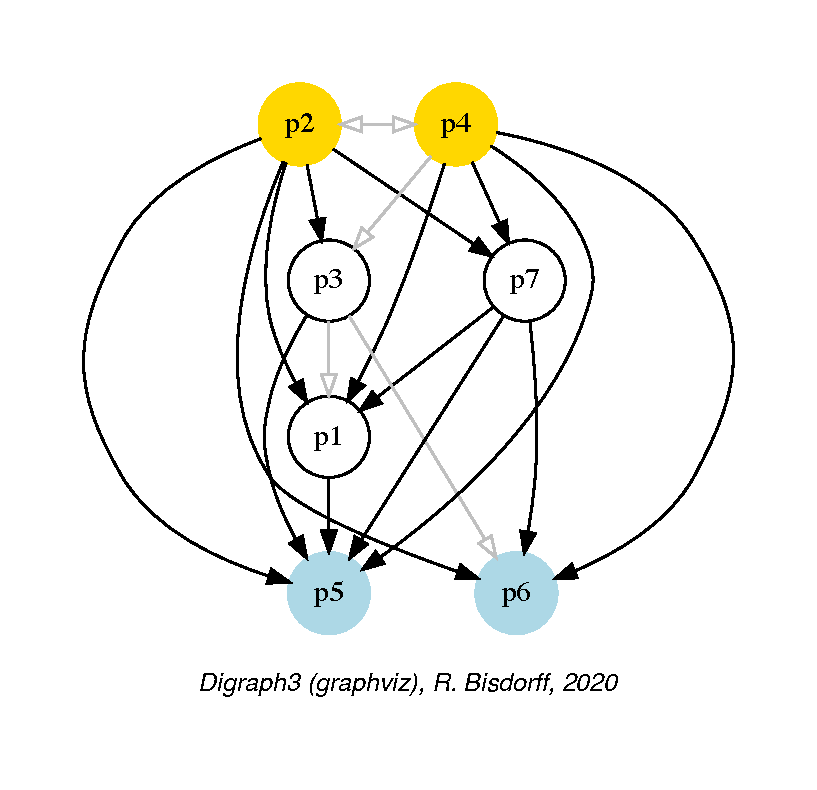
\includegraphics[height=6cm]{Figures/19-1-stdg.pdf}\hfill
  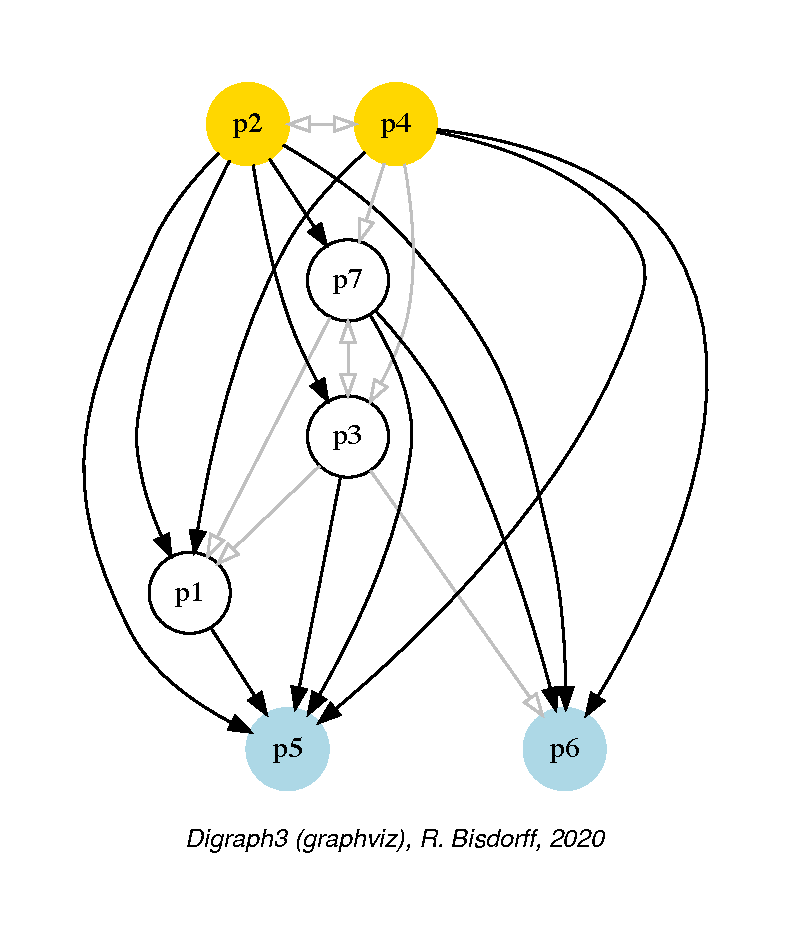
\includegraphics[height=6cm]{Figures/19-1-robg.pdf}
\caption{\emph{Standard} versus \emph{robust} strict outranking digraphs oriented by their initial and terminal prekernels} 
\label{fig:19.1}       % Give a unique label
\end{figure}
   
The robust version (right in Fig.~\vref{fig:19.1}) drops two strict outranking situations: between \texttt{p4} and \texttt{p7} and between \texttt{p7} and \texttt{p1}. The remaining 14 strict outranking (resp. outranked) situations are now all verified at a stability level of $+2$ and more (resp. $-2$ and less). They remain valid, hence, with all potential significance weights that are compatible with the given significance weights preordering (see List.~\vref{list:19.2}).

To appreciate the apparent partial ordering of both the standard and the robust strict outranking digraphs shown in Figure~\vref{fig:19.1}, let us have a final heatmap view in Figure~\vref{fig:19.2} on the underlying performance tableau ordered by the \NetFlows ranking rule actually applied to the robust version of the outranking digraph (see the \texttt{outrankingModel='this'} flag in Line 4 below).
\begin{lstlisting}[caption={Computing a robust performance heatmap view},label=list:19.9]
>>> rg.showHTMLPerformanceHeatmap(\
...           Correlations=True,\
...           colorLevels=5,\
...           outrankingModel='this',\
...           rankingRule='NetFlows')
\end{lstlisting}
\begin{figure}[ht]
%\sidecaption
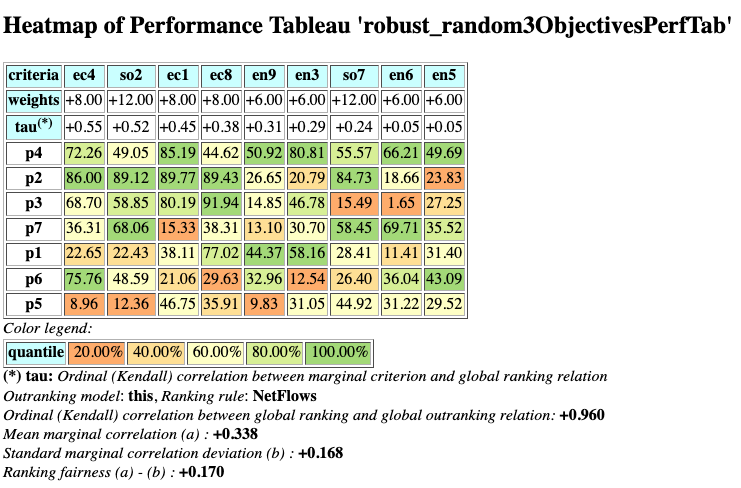
\includegraphics[width=\hsize]{Figures/19-2-robustHeatmap.png}
\caption{Robust heatmap of the random 3 objectives performance tableau ordered by the \NetFlows ranking rule} 
\label{fig:19.2}       % Give a unique label
\end{figure}

As the initial prekernel \{\texttt{p2}, \texttt{p4}\} is in the robust outranking digraph validated at least at stability level $\pm 2$, recommending alternatives \texttt{p4}, as well as \texttt{p2}, as potential best choices, appears robustly justified. Alternative \texttt{p4} represents indeed an overall \emph{best compromise choice} between all decision objectives, whereas alternative \texttt{p2} gives an unanimous best choice with respect to two out of three decision objectives. Up to the decision maker to make his final choice.

\section{Characterising unopposed multiobjective outranking situations}
\label{sec:19.5}

When facing a performance tableau involving multiple decision objectives, the robustness level $\pm 3$  may lead to distinguishing what we call \emph{unopposed} outranking situations, like the one shown in the previous section between alternative \texttt{p4} and \texttt{p1} ($r(p4 \succsim p1) = +0.78$, see List.~\vref{list:19.4} Line 11), namely preferential situations that are more or less validated or invalidated by all the decision objectives.  

\begin{definition}[Unopposed outranking situation]\label{def:19.2}
\begin{itemize}
\item We say that decision alternative \texttt{x} \emph{unopposedly outranks} decision alternative \texttt{y} when  \texttt{x} positively outranks \texttt{y} on one or more decision objectives without \texttt{x} being positively outranked by \texttt{y} on any decision objective.
\item Dually, we say that decision alternative \texttt{x} \emph{is unopposedly outranked by} decision alternative \texttt{y} when \texttt{x} is positively outranked by \texttt{y} on one or more decision objectives without \texttt{x} positively outranking \texttt{y} on any decision objective.
\end{itemize}
\end{definition}

Let us reconsider, for instance, the performance tableau \texttt{pt} with three decision objectives already seen in Listing~\vref{list:19.1}:
\begin{lstlisting}
>>> pt.showObjectives()
  *------ show objectives -------"
   Eco: Economical aspect
     ec1 criterion of objective Eco 8
     ec4 criterion of objective Eco 8
     ec8 criterion of objective Eco 8
    Total weight: 24.00 (3 criteria)
   Soc: Societal aspect
     so2 criterion of objective Soc 12
     so7 criterion of objective Soc 12
    Total weight: 24.00 (2 criteria)
   Env: Environmental aspect
     en3 criterion of objective Env 6
     en5 criterion of objective Env 6
     en6 criterion of objective Env 6
     en9 criterion of objective Env 6
    Total weight: 24.00 (4 criteria)
\end{lstlisting}

We notice in this example three decision objectives of equal importance (see Lines 3,13,17). What will be the outranking situations that are positively (resp.  negatively) validated for each one of the decision objectives taken individually ?

We may obtain such unopposed multiobjective outranking situations by operating an epistemic \emph{average fusion} (see the \texttt{symmetricAverage()} method\index{symmetricAverage@\texttt{symmetricAverage()}}) of the marginal outranking digraphs restricted to the coalition of criteria supporting each one of the decision objectives (see List.~\vref{list:19.9}).
\begin{lstlisting}[caption={Computing unopposed outranking situations},label=list:19.9]
>>> from outrankingDigraphs import\
...                     BipolarOutrankingDigraph
>>> geco = BipolarOutrankingDigraph(pt,\
...                     objectivesSubset=['Eco'])
>>> gsoc = BipolarOutrankingDigraph(pt,\
...                     objectivesSubset=['Soc'])
>>> genv = BipolarOutrankingDigraph(pt,\
...                     objectivesSubset=['Env'])
>>> from digraphs import FusionLDigraph
>>> objectiveWeights = \
...               [pt.objectives[obj]['weight']\
...                      for obj in t.objectives] 
>>> uopg = FusionLDigraph([geco,gsoc,genv],\
...                   operator='o-average',\
...                   weights=objectiveWeights)
>>> uopg.showRelationTable(ReflexiveTerms=False)
  * ---- Relation Table -----
   r   |  'p1'   'p2'   'p3'   'p4'   'p5'   'p6'   'p7'   
  -----|------------------------------------------------
  'p1' |    -   +0.00  +0.00  -0.69  +0.39  +0.11  +0.00  
  'p2' | +0.00    -    +0.83  +0.00  +0.00  +0.00  +0.00  
  'p3' | +0.00  -0.33    -    +0.00  +0.50  +0.00  +0.00  
  'p4' | +0.78  +0.00  +0.61    -    +1.00  +1.00  +0.67  
  'p5' | -0.11  +0.00  +0.00  -0.89    -    +0.11  +0.00  
  'p6' | +0.00  +0.00  +0.00  -0.44  +0.17    -    +0.00  
  'p7' | +0.00  +0.00  +0.00  +0.00  +0.78  +0.42    -   
  Valuation domain: [-1.0; 1.0]
\end{lstlisting}

Positive (resp. negative) $r(x \succsim y)$ characteristic values, like $r(p1 \succsim p5) = +0.39$ (see List.~\vref{list:19.9} Line 20), show hence only outranking situations being validated (resp. invalidated) by one or more decision objectives without being invalidated (resp. validated) by any other decision objective.

For easily computing this kind of \emph{unopposed multiobjective} outranking digraphs, the \texttt{outrankingDigraphs} module conveniently provides a corresponding\\ \texttt{UnOpposedBipolarOutrankingDigraph} constructor \index{UnOpposedBipolarOutrankingDigraph@\texttt{UnOpposedBipolarOutrankingDigraph} class}.
\begin{lstlisting}[caption={Computing unopposed outranking digraphs},label=list:19.10]
>>> from outrankingDigraphs import\
...              UnOpposedBipolarOutrankingDigraph
>>> uopg = UnOpposedBipolarOutrankingDigraph(pt)
>>> uopg
  *------- Object instance description ------*
   Instance class      : UnOpposedBipolarOutrankingDigraph
   Instance name       : unopposed_outrankings
   Actions           : 7
   Criteria          : 9
   Size                : 13
   Oppositeness (%)    : 43.48
   Determinateness (%) : 61.71
   Valuation domain    : [-1.00;1.00]
   Attributes          : ['name', 'actions',
                'valuationdomain', 'objectives',
                'criteria', 'methodData',
                'evaluation', 'order', 'runTimes',
                'relation', ...
                'gamma', 'notGamma']
>>> uopg.computeOppositeness(InPercents=True)
  {'standardSize': 23, 'unopposedSize': 13,
   'oppositeness': 43.47826086956522}			   
\end{lstlisting}

The resulting \emph{unopposed} outranking digraph keeps in fact 13 (see List.\vref{list:19.10} Lines 20-22) out of the 23 positively validated \emph{standard} outranking situations, leading to a degree of \emph{oppositeness} --preferential disagreement between decision objectives-- of $(1.0 - 13/23)\,=\,0.4348$.

We may now, for instance, verify the unopposed status of the outranking situation observed between alternatives \texttt{p1} and \texttt{p5}.
\begin{lstlisting}[caption={Example of unopposed multiobjective outranking situation},label=list:19.11]
>>> uopg.showPairwiseComparison('p1','p5')
 *------------  pairwise comparison ----*
  Comparing actions : ('p1', 'p5')
  crit. wght.  g(x)  g(y)    diff   | ind   pref     r()
  ec1   8.00  38.11  46.75  -8.64   | 5.00  10.00   +0.00
  ec4   8.00  22.65  8.96  +13.69   | 5.00  10.00   +8.00
  ec8   8.00  77.02  35.91  +41.11  | 5.00  10.00   +8.00
  en3   6.00  58.16  31.05  +27.11  | 5.00  10.00   +6.00
  en5   6.00  31.40  29.52  +1.88   | 5.00  10.00   +6.00
  en6   6.00  11.41  31.22  -19.81  | 5.00  10.00   -6.00
  en9   6.00  44.37  9.83  +34.54   | 5.00  10.00   +6.00
  so2   12.00  22.43  12.36  +10.07 | 5.00  10.00  +12.00
  so7   12.00  28.41  44.92  -16.51 | 5.00  10.00  -12.00
  Valuation in range: -72.00 to +72.00;           -------
                               global concordance: +28.00
\end{lstlisting}

In Listing~\vref{list:19.11} we see that alternative \texttt{p1} does indeed positively outrank alternative \texttt{p5} from the economic perspective ($r(p1 \succsim_{Eco} p5) = +16/24$) as well as from the environmental perspective ($r(p1 \succsim_{Env} p5) = +12/24$). Whereas, from the societal perspective, both alternatives appear incomparable ($r(p1 \succsim_{Soc} p5) = 0/24$).

When proportionally equal criteria significance weights per objective are given, these outranking situations appear hence \emph{stable} with respect to all possible importance weights we could allocate to the decision objectives.

This gives way for computing multiobjective \emph{Pareto efficient} choice recommendations. 

\section{Computing Pareto efficient multiobjective choices}
\label{sec:19.6}

Indeed, best choice recommendations, computed from an \emph{unopposed multiobjective} outranking digraph, deliver the case given \emph{Pareto efficient} choices. 
\begin{lstlisting}[caption={Pareto efficient multiobjective choice},label=list:19.12]
>>> uopg.showBestChoiceRecommendation()
  Best choice recommendation(s) (BCR)
   (in decreasing order of determinateness)   
   Credibility domain: [-1.00,1.00]
   === >> potential first choice(s)
   choice              : ['p2', 'p4', 'p7']
      independence        : 0.00
      dominance           : 0.33
      absorbency          : 0.00
      covering (%)        : 33.33
      determinateness (%) : 50.00
   === >> potential last choice(s) 
   choice              : ['p3', 'p5', 'p6', 'p7']
      independence        : 0.00
      dominance           : -0.61
      absorbency          : 0.11
      covered (%)         : 33.33
      determinateness (%) : 50.00
\end{lstlisting}

Our previous \emph{robust} best choice recommendation (\texttt{p2} and \texttt{p4}, see Fig.~\vref{fig:19.1}) remains, in this example here, \emph{stable}. We recover indeed the best choice recommendation [\texttt{p2}, \texttt{p4}, \texttt{p7}] (see List.~\vref{list:19.12} Line 6). Yet, notice that decision alternative \texttt{p7} appears to be at the same time a potential \emph{first} as well as a potential \emph{last} choice recommendation (see Line 13), a consequence of \texttt{p7} being completely \emph{incomparable} to the other decision alternatives when restricting the comparability to only unopposed strict outranking situations. 

This kind of Pareto efficient result is shown in Figure~\vref{fig:19.3}.
\begin{lstlisting}
>>> (~(-uopg)).exportGraphViz(fileName = 'unopDigraph',\
...                           firstChoice = ['p2','p4'],\
...                           lastChoice = ['p3','p5','p6'])
  *---- exporting a dot file for GraphViz tools ----*
   Exporting to unopDigraph.dot
   dot -Grankdir=BT -Tpng unopDigraph.dot -o unopDigraph.png
\end{lstlisting}
\begin{figure}[ht]
%\sidecaption
  Standard strict outranking digraph \hfill Unopposed strict outranking digraph \\
  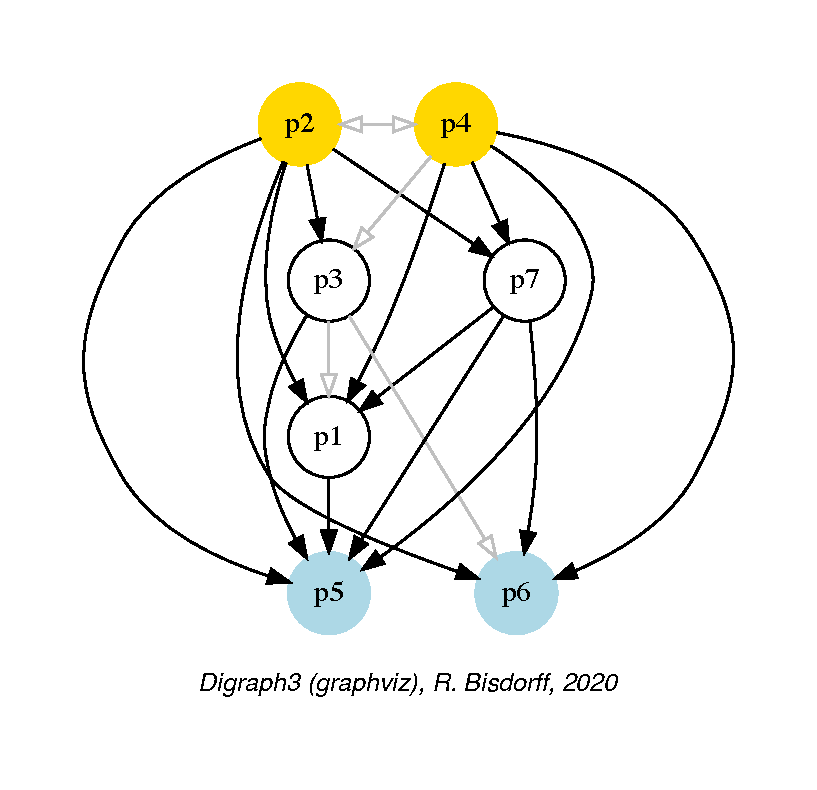
\includegraphics[height=6cm]{Figures/19-1-stdg.pdf}\hfill
  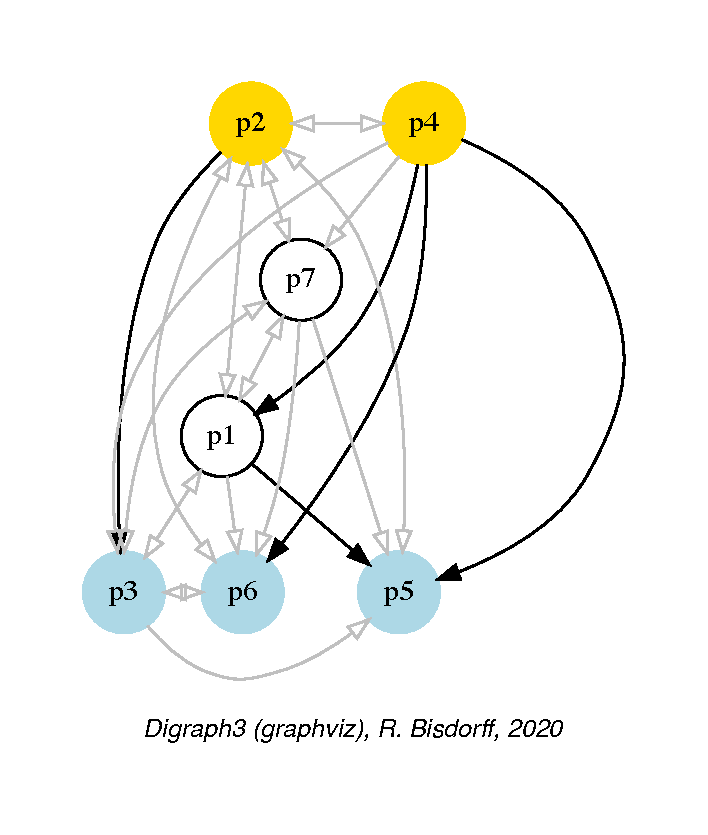
\includegraphics[height=6cm]{Figures/19-3-unopDigraph.pdf}
\caption{Standard versus \emph{unopposed} strict outranking digraphs oriented by first and last choice recommendations} 
\label{fig:19.3}       % Give a unique label
\end{figure}

In order to make now an eventual best unique choice, a decision maker will necessarily have to weigh, in a second stage of the decision aiding process, the relative importance of the individual decision objectives.

In a \emph{social choice} context, where decision objectives would match different political parties, Pareto efficient best choice recommendations represent in fact \emph{multipartisan} social choices that may judiciously temper plurality tyranny effects. This idea is developed in the following Chapter~\ref{sec:20}.

\vspace{1cm}

For concluding, let us mention that it is precisely again our bipolar-valued logical characteristic framework that provides us here with a first order distributional dominance test for effectively qualifying the stability level $\pm 2$ robustness of an outranking digraph when facing performance tableaux with criteria of only ordinal-valued significance. A real-world application of our stability analysis with such a kind of performance tableau may be consulted in \citep{BIS-2015bestPoster}.



%%%%%%% The chapter bibliography
%\normallatexbib
%\clearpage
%\phantomsection
%\addcontentsline{toc}{section}{Chapter Bibliography}
\chapter[On robust outrankings]{Robustness analysis of outranking digraphs}
\label{sec:19}

\abstract*{ The required cardinal significance weights of the performance criteria represent the '\emph{Achilles}' heel of our outranking approach. Rarely will indeed a decision maker be cognitively competent for suggesting precise decimal-valued criteria significance weights. More often, the decision problem will involve more or less equally important decision objectives with more or less equi-significant criteria.
In this chapter, we study the stability of the outranking digraph when the criteria significance weights faithfully indicate solely an order of importance.}

\abstract{ The required cardinal significance weights of the performance criteria represent the '\emph{Achilles}' heel of our outranking approach. Rarely will indeed a decision maker be cognitively competent for suggesting precise decimal-valued criteria significance weights. More often, the decision problem will involve more or less equally important decision objectives with more or less equi-significant criteria.
In this chapter, we study the stability of the outranking digraph when the criteria significance weights faithfully indicate solely an order of importance.}

\section{Cardinal or ordinal criteria significance weights}
\label{sec:19.1}

A random example of such a decision problem with equally important decision objectives and equi-significant criteria may be generated with the \texttt{Random3\-Objectives\-PerformanceTableau} class \index{Random3ObjectivesPerformanceTableau@\texttt{Random3ObjectivesPerformanceTableau()}}.

\begin{lstlisting}[caption={Generate a Random 3 Objectives Performance Tableau},label=list:19.1]
>>> from randomPerfTabs import \
...           Random3ObjectivesPerformanceTableau
>>> pt = Random3ObjectivesPerformanceTableau(\
...           numberOfActions=7,\
...           numberOfCriteria=9,seed=102)
>>> pt
    *------- PerformanceTableau instance description ------*
    Instance class   : Random3ObjectivesPerformanceTableau
    Seed             : 102
    Instance name    : random3ObjectivesPerfTab
    Actions          : 7
    Objectives       : 3
    Criteria         : 9
    NA proportion (%): 0.0
    Attributes       : ['name', 'valueDigits', 'BigData',
              'OrdinalScales', 'missingDataProbability',
              'negativeWeightProbability', 'randomSeed',
              'sumWeights', 'valuationPrecision',
              'commonScale', 'objectiveSupportingTypes',
              'actions', 'objectives', 'criteriaWeightMode',
              'criteria', 'evaluation', 'weightPreorder']
>>> pt.showObjectives()
  *------ show objectives -------*
   Eco: Economical aspect
     ec1 criterion of objective Eco 8
     ec4 criterion of objective Eco 8
     ec8 criterion of objective Eco 8
     Total weight: 24.00 (3 criteria)
   Soc: Societal aspect
     so2 criterion of objective Soc 12
     so7 criterion of objective Soc 12
     Total weight: 24.00 (2 criteria)
   Env: Environmental aspect
     en3 criterion of objective Env 6
     en5 criterion of objective Env 6
     en6 criterion of objective Env 6
     en9 criterion of objective Env 6
     Total weight: 24.00 (4 criteria)
\end{lstlisting}
In Listing~\ref{list:19.1} one may notice a performance tableau \texttt{pt} describing seven decision alternatives that are assessed with respect to three equally important decision objectives concerning: --first, an \emph{economical} aspect (Line 24) with a coalition of three performance criteria of significance weight 8, --secondly, a \emph{societal} aspect (Line 29) with a coalition of two performance criteria of significance weight 12, and --thirdly, an \emph{environmental} aspect (Line 33) with a coalition four performance criteria of significance weight 6.

The question we tackle is the following: How \emph{dependent} on the actual values of the significance weights appears to be the corresponding bipolar-valued outranking digraph ? In the previous Chapter~\ref{sec:18} we assumed that the criteria significance weights were random variables. Here, we shall assume that we know for sure only the preordering of the significance weights. In our example we see indeed three increasing weight equivalence classes.
\begin{lstlisting}[caption={The significance weights preorder},label=list:19.2]
>>> pt.showWeightPreorder()
    ['en3', 'en5', 'en6', 'en9'] (6) <
    ['ec1', 'ec4', 'ec8'] (8) <
    ['so2', 'so7'] (12)
\end{lstlisting}
How stable appear now to be the outranking situations when allowing all possible significance weights that are compatible with this weights preorder shown in Listing~\ref{list:19.2} ?

\section{Qualifying the stability of outranking situations}
\label{sec:19.2}

Let us construct the bipolar-valued outranking digraph corresponding to the random 3-Objectives performance tableau \texttt{pt}.
\begin{lstlisting}[caption={Example Bipolar Outranking Digraph},label=list:19.3]
>>> from outrankingDigraphs import BipolarOutrankingDigraph
>>> g = BipolarOutrankingDigraph(pt)
>>> g.showRelationTable()
  * ---- Relation Table -----
   r(>=) |  'p1'   'p2'   'p3'   'p4'   'p5'   'p6'   'p7'   
   ------|------------------------------------------------
    'p1' | +1.00  -0.42  +0.00  -0.69  +0.39  +0.11  -0.06  
    'p2' | +0.58  +1.00  +0.83  +0.00  +0.58  +0.58  +0.58  
    'p3' | +0.25  -0.33  +1.00  +0.00  +0.50  +1.00  +0.25  
    'p4' | +0.78  +0.00  +0.61  +1.00  +1.00  +1.00  +0.67  
    'p5' | -0.11  -0.50  -0.25  -0.89  +1.00  +0.11  -0.14  
    'p6' | +0.22  -0.42  +0.00  -1.00  +0.17  +1.00  -0.11  
    'p7' | +0.22  -0.50  +0.17  -0.06  +0.78  +0.42  +1.00  
\end{lstlisting}
In Listing~\ref{list:19.3} Lines 7-13, we notice on the principal diagonal of the relation table the certainly validated reflexive terms $+1.00$ that are trivially independent of any significance weights. Now, we know for sure that \emph{unanimous} outranking situations are also completely independent of the significance weights. And, all outranking situations that are supported by a majority significance in each coalition of equi-significant criteria are as well independent of the actual importance we attach to each individual criteria coalition. We are furthermore able to effectively test if an outranking situation is in fact independent of all the potential significance weights that are compatible with the given preordering of the weights shown in Listing \ref{list:19.2} \citep{BIS-2014}. Mind that usually one also obtains outranking situations that are \emph{dependent} on the precise cardinal weights we allocate to the criteria significances.

Such a stability denotation of outranking situations may be inspected by using the \texttt{StabilityDenotation=True} flag \index{StabilityDenotation@\texttt{StabilityDenotation} flag} with the common \texttt{showRelationTable()} method.
\begin{lstlisting}[caption={Bipolar-valued outranking relation table with stability denotation},label=list:19.4]
>>> g.showRelationTable(StabilityDenotation=True)
  * ---- Relation Table -----
   r/(stab)  |  'p1'  'p2'  'p3'  'p4'  'p5'  'p6'  'p7'   
   ----------|------------------------------------------
     'p1'    | +1.00 -0.42 +0.00 -0.69 +0.39 +0.11 -0.06  
             |  (+4)  (-2)  (+0)  (-3)  (+2)  (+2)  (-1)  
     'p2'    | +0.58 +1.00 +0.83  0.00 +0.58 +0.58 +0.58  
             |  (+2)  (+4)  (+3)  (+2)  (+2)  (+2)  (+2)  
     'p3'    | +0.25 -0.33 +1.00  0.00 +0.50 +1.00 +0.25  
             |  (+2)  (-2)  (+4)   (0)  (+2)  (+2)  (+1)  
     'p4'    | +0.78  0.00 +0.61 +1.00 +1.00 +1.00 +0.67  
             |  (+3)  (-1)  (+3)  (+4)  (+4)  (+4)  (+2)  
     'p5'    | -0.11 -0.50 -0.25 -0.89 +1.00 +0.11 -0.14  
             |  (-2)  (-2)  (-2)  (-3)  (+4)  (+2)  (-2)  
     'p6'    | +0.22 -0.42  0.00 -1.00 +0.17 +1.00 -0.11
             |  (+2)  (-2)  (+1)  (-2)  (+2)  (+4)  (-2)  
     'p7'    | +0.22 -0.50 +0.17 -0.06 +0.78 +0.42 +1.00  
             |  (+2)  (-2)  (+1)  (-1)  (+3)  (+2)  (+4)  
\end{lstlisting}
In Listing~\ref{list:19.4} we may hence distinguish the following bipolar-valued stability levels:
\begin{itemize}[leftmargin=1cm]
\item [$\mathbf{\pm 4}$:] \emph{unanimous} outranking, resp. outranked situation. The pairwise trivial reflexive outrankings, for instance, all show this stability level;
\item [$\mathbf{\pm 3}$:] validated outranking, resp. outranked situation in \emph{each} coalition of equisignificant criteria. This is, for instance, the case for the outranking situation observed between alternatives \texttt{p1} and \texttt{p4} (see Listing \ref{list:19.4} Lines 6 and 12);
\item [$\mathbf{\pm 2}$:] validated outranking, resp. outranked situation with \emph{all} potential significance weights that are \emph{compatible} With the given significance preorder (see Listing \ref{list:19.2}). This is the case when comparing alternatives \texttt{p1} and \texttt{p2} (see Lines 6 and 8);
\item [$\mathbf{\pm 1}$:] validated outranking, resp. outranked situation with the \emph{precisely given decimal} significance weights, a situation we may observe between alternatives \texttt{p3} and \texttt{p7} (see Lines 10 and 16);
\item [$\mathbf{0}$:] \texttt{indeterminate} outranking situation, like the one between alternatives \texttt{p1} and \texttt{p3} (see Lines 6 and 10).
\end{itemize}

It is worthwhile noticing that, in the one limit case where all performance criteria appear equi-significant, i.e. there is given a single equivalence class containing all the criteria significance weights, one may only distinguish stability levels $\pm 4$ and $\pm 3$. In the other limit case, when all performance criteria admit different significanceweights, i.e. the significance weights may be linearly ordered without ties and no stability level $+3$ or $-3$ may be observed.

As mentioned above, all reflexive comparisons trivially confirm an unanimous outranking situation: all decision alternatives are indeed always``\emph{performing as well as}'' themselves. But there appear also two non reflexive unanimous outranking situations: when comparing, for instance, alternative \texttt{p4} with alternatives \texttt{p5} and \texttt{p6} (see Listing \ref{list:19.4} Lines 14 and 16). Let us inspect the details of how alternatives \texttt{p4} and \texttt{p5} compare.
\begin{lstlisting}
>>> g.showPairwiseComparison('p4','p5')
 *------------  pairwise comparison ----*
  Comparing actions : (p4, p5)
  crit. wght.  g(x)  g(y)    diff  | ind   pref    r()
  ec1   8.00  85.19  46.75  +38.44 | 5.00  10.00   +8.00
  ec4   8.00  72.26   8.96  +63.30 | 5.00  10.00   +8.00
  ec8   8.00  44.62  35.91   +8.71 | 5.00  10.00   +8.00
  en3   6.00  80.81  31.05  +49.76 | 5.00  10.00   +6.00
  en5   6.00  49.69  29.52  +20.17 | 5.00  10.00   +6.00
  en6   6.00  66.21  31.22  +34.99 | 5.00  10.00   +6.00
  en9   6.00  50.92   9.83  +41.09 | 5.00  10.00   +6.00
  so2  12.00  49.05  12.36  +36.69 | 5.00  10.00  +12.00
  so7  12.00  55.57  44.92  +10.65 | 5.00  10.00  +12.00
  Valuation in range: -72.00 to +72.00;          -------
                             global concordance:  +72.00
\end{lstlisting}
Alternative \texttt{p4} is indeed performing unanimously ``\emph{at least as well as}'' alternative \texttt{p5} and $r(p4 \succsim p5)\; =\; 72/72\; =\; +1.00$ (see Listing \ref{list:19.4} Line 11).

The converse comparison does not, however, deliver such an unanimous outranked situation. 
\begin{lstlisting}
>>> g.showPairwiseComparison('p5','p4')
 *------------  pairwise comparison ----*
  Comparing actions : (p5, p4)
  crit. wght.  g(x)  g(y)    diff  | ind   pref     r()
  ec1   8.00  46.75  85.19  -38.44 | 5.00  10.00   -8.00
  ec4   8.00   8.96  72.26  -63.30 | 5.00  10.00   -8.00
  ec8   8.00  35.91  44.62   -8.71 | 5.00  10.00   +0.00
  en3   6.00  31.05  80.81  -49.76 | 5.00  10.00   -6.00
  en5   6.00  29.52  49.69  -20.17 | 5.00  10.00   -6.00
  en6   6.00  31.22  66.21  -34.99 | 5.00  10.00   -6.00
  en9   6.00   9.83  50.92  -41.09 | 5.00  10.00   -6.00
  so2  12.00  12.36  49.05  -36.69 | 5.00  10.00  -12.00
  so7  12.00  44.92  55.57  -10.65 | 5.00  10.00  -12.00
  Valuation in range: -72.00 to +72.00;           ------
                             global concordance:  -64.00
\end{lstlisting}
The converse comparison only qualifies at stability level $-3$ (see Listing \ref{list:19.4} Line 13); $r(p5 \succsim p4)\; =\; -64/72\; =\; -0.89$). On criterion \texttt{ec8} we observe indeed a small negative performance difference of $-8.71$ (see Line 7 above) which is effectively below the supposed preference discrimination threshold of $10.00$. Yet, the outranked situation is supported by a majority of criteria in each decision objective. Hence, the reported preferential situation is completely independent of any chosen significance weights.

Let us now consider a comparison, like the one between alternatives \texttt{p2} and \texttt{p1}, that is qualified at stability level $+2$, resp. $-2$.
\begin{lstlisting}[caption={Comparison of alternatives \texttt{p2} and \texttt{p1}},label=list:19.5]
>>> g.showPairwiseOutrankings('p2','p1')
  *------------  pairwise comparison ----*
   Comparing actions : (p2, p1)
   crit. wght.  g(x)  g(y)    diff  | ind   pref     r()
   ec1   8.00  89.77  38.11  +51.66 | 5.00  10.00   +8.00
   ec4   8.00  86.00  22.65  +63.35 | 5.00  10.00   +8.00
   ec8   8.00  89.43  77.02  +12.41 | 5.00  10.00   +8.00
   en3   6.00  20.79  58.16  -37.37 | 5.00  10.00   -6.00
   en5   6.00  23.83  31.40   -7.57 | 5.00  10.00   +0.00
   en6   6.00  18.66  11.41   +7.25 | 5.00  10.00   +6.00
   en9   6.00  26.65  44.37  -17.72 | 5.00  10.00   -6.00
   so2  12.00  89.12  22.43  +66.69 | 5.00  10.00  +12.00
   so7  12.00  84.73  28.41  +56.32 | 5.00  10.00  +12.00
   Valuation in range: -72.00 to +72.00;          -------
                              global concordance:  +42.00
    *------------  pairwise comparison ----*
    Comparing actions : ('p1', 'p2')
    crit. wght.  g(x)  g(y)    diff  | ind   pref     r()
    ec1   8.00  38.11  89.77  -51.66 | 5.00  10.00   -8.00
    ec4   8.00  22.65  86.00  -63.35 | 5.00  10.00   -8.00
    ec8   8.00  77.02  89.43  -12.41 | 5.00  10.00   -8.00
    en3   6.00  58.16  20.79  +37.37 | 5.00  10.00   +6.00
    en5   6.00  31.40  23.83   +7.57 | 5.00  10.00   +6.00 
    en6   6.00  11.41  18.66   -7.25 | 5.00  10.00   +0.00
    en9   6.00  44.37  26.65  +17.72 | 5.00  10.00   +6.00
    so2  12.00  22.43  89.12  -66.69 | 5.00  10.00  -12.00
    so7  12.00  28.41  84.73  -56.32 | 5.00  10.00  -12.00
    Valuation in range: -72.00 to +72.00;          -------
                                global concordance: -30.00
\end{lstlisting}
In both comparisons, the performances observed with respect to the environmental decision objective are not validating with a significant majority the outranking, resp. outranked situation. Hence, the stability of the reported preferential situations is in fact dependent on choosing significance weights that are compatible with the given significance weights preorder (see Listing \ref{list:19.2}).

Let us finally inspect a comparison that is only qualified at stability level $+1$, like the one between alternatives \texttt{p7} and \texttt{p3}.
\begin{lstlisting}[caption={Comparison of alternatives \texttt{p7} and \texttt{p3}},label=list:19.6]
>>> g.showPairwiseOutrankings('p7','p3')
 *------------  pairwise comparison ----*
  Comparing actions : ('p7', 'p3')
  crit. wght.  g(x)  g(y)    diff  | ind   pref     r()
  ec1   8.00  15.33  80.19  -64.86 | 5.00  10.00   -8.00
  ec4   8.00  36.31  68.70  -32.39 | 5.00  10.00   -8.00
  ec8   8.00  38.31  91.94  -53.63 | 5.00  10.00   -8.00
  en3   6.00  30.70  46.78  -16.08 | 5.00  10.00   -6.00
  en5   6.00  35.52  27.25   +8.27 | 5.00  10.00   +6.00
  en6   6.00  69.71   1.65  +68.06 | 5.00  10.00   +6.00
  en9   6.00  13.10  14.85   -1.75 | 5.00  10.00   +6.00
  so2  12.00  68.06  58.85   +9.21 | 5.00  10.00  +12.00
  so7  12.00  58.45  15.49  +42.96 | 5.00  10.00  +12.00
  Valuation in range: -72.00 to +72.00;          -------
                              global concordance: +12.00
 *------------  pairwise comparison ----*
  Comparing actions : ('p3', 'p7')
  crit. wght.  g(x)  g(y)    diff  | ind   pref     r()
  ec1   8.00  80.19  15.33  +64.86 | 5.00  10.00   +8.00
  ec4   8.00  68.70  36.31  +32.39 | 5.00  10.00   +8.00
  ec8   8.00  91.94  38.31  +53.63 | 5.00  10.00   +8.00
  en3   6.00  46.78  30.70  +16.08 | 5.00  10.00   +6.00
  en5   6.00  27.25  35.52   -8.27 | 5.00  10.00   +0.00
  en6   6.00   1.65  69.71  -68.06 | 5.00  10.00   -6.00
  en9   6.00  14.85  13.10   +1.75 | 5.00  10.00   +6.00
  so2  12.00  58.85  68.06   -9.21 | 5.00  10.00   +0.00
  so7  12.00  15.49  58.45  -42.96 | 5.00  10.00  -12.00
  Valuation in range: -72.00 to +72.00;          -------
                              global concordance: +18.00
\end{lstlisting}
In both cases, choosing only significances that are compatible with the given weights preorder will not always result in positively validated outranking situations.

\section{Computing the stability denotation of outranking situations}
\label{sec:19.3}

Stability levels $\pm 4$ and $\pm 3$ are, the case given, easy to detect. Detecting a stability level $\pm 2$ is far less obvious.  Now, it is precisely again the bipolar-valued epistemic characteristic domain that will give us a way to implement an effective test for stability level $+2$ and $-2$ \citep{BIS-2004b,BIS-2004c}. 

Let us consider the significance equivalence classes we observe in the given weights preorder. Here we observe three weight classes: $6$, $8$, and $12$, in increasing order (see Listing \ref{list:19.2}). In the pairwise comparisons, shown above, these equivalence classes may appear positively or negatively, besides the indeterminate significance of value $0.00$. We thus get the following ordered bipolar list of significance weights: $W = [-12. -8. -6, 0, 6, 8, 12]$.

In all the pairwise marginal comparisons shown in the previous Section, we may observe that each one of the nine criteria assigns one precise item out of this list $W$. Let us denote $q[i]$ the number of criteria assigning item $W[i]$, and $Q[i]$ the cumulative sums of these $q[i]$ counts, where $i$ is an index in the range of the length of list $W$.

In the comparison of alternatives \texttt{p2} and \texttt{p1}, for instance (see Listing \ref{list:19.5}), we observe the following counts: \hfill
\begin{center}
\begin{tabular}{l|r|r|r|r|r|r|r}
 \svhline\noalign{\smallskip}
  $W[i]$ & -12 & -8  & -6  &  0  &  6  &  8 &  12\\  
 \noalign{\smallskip}\hline\noalign{\smallskip}
$q[i]$  &  0 &  0 &   2 &   1  &  1  &  3  &  2 \\
$Q[i]$  &  0 &  0 &   2 &   3  &  4  &  7  &  9 \\
      \noalign{\smallskip}\hline
\end{tabular}
\end{center}

\noindent Let use denote $-q$ and $-Q$ the reversed versions of the $q$ and the $Q$ lists. We thus obtain the following result.\hfill
\begin{center}
\begin{tabular}{l|r|r|r|r|r|r|r}
 \svhline\noalign{\smallskip}
  $W[i]$ & -12 & -8  & -6  &  0  &  6  &  8 &  12\\  
 \noalign{\smallskip}\hline\noalign{\smallskip}
  $-q[i]$  &  2 &  3 &   1 &   1  &  2  &  0  &  0 \\
  $-Q[i]$  &  2 &  5 &   6 &   7  &  9  &  9  &  9 \\
 \noalign{\smallskip}\hline
\end{tabular}
\end{center}

Now, a pairwise outranking situation will be qualified at stability level $+2$, i.e. positively validated with any significance weights that are compatible with the given weights preorder, when for all $i$, we observe $Q[i] \leq -Q[i]$ and there exists one $i$ such that $Q[i] < -Q[i]$. Similarly, a pairwise outranked situation will be qualified at stability level $-2$, when for all $i$, we observe $Q[i] \geq -Q[i]$ and there exists one $i$ such that $Q[i] > -Q[i]$ \citep{BIS-2004c}.

We may verify, for instance, that the outranking situation observed between alternatives \texttt{p2} and \texttt{p1} does indeed verify this \emph{first order distributional dominance} condition. \hfill
\begin{center}
\begin{tabular}{l|r|r|r|r|r|r|r}
 \svhline\noalign{\smallskip}
  $W[i]$ & -12 & -8  & -6  &  0  &  6  &  8 &  12\\  
 \noalign{\smallskip}\hline\noalign{\smallskip}
  $Q[i]$  &  0 &  0 &   2 &   3  &  4  &  7  &  9 \\
  $-Q[i]$  &  2 &  5 &   6 &   7  &  9  &  9  &  9 \\
 \noalign{\smallskip}\hline
\end{tabular}
\end{center}

Notice that outranking situations qualified at stability levels $\pm 4$ and $\pm 3$, evidently also verify the stability level $\pm 2$ test above. The outranking situation between alternatives \texttt{p7} and \texttt{p3} does not, however, verify this test (see Listing \ref{list:19.6}).\hfill
\begin{center}
\begin{tabular}{l|r|r|r|r|r|r|r}
 \svhline\noalign{\smallskip}
  $W[i]$ & -12 & -8  & -6  &  0  &  6  &  8 &  12\\  
 \noalign{\smallskip}\hline\noalign{\smallskip}
  $q[i]$  &  0 &  3 &   1 &   0  &  3  &  0  &  2 \\
  $Q[i]$  &  0 &  3 &   4 &   4  &  7  &  7  &  9 \\
  $-Q[i]$  &  2 &  2 &   5 &   5  &  6  &  9  &  9 \\
 \noalign{\smallskip}\hline
\end{tabular}
\end{center}
This time, not all the $Q[i]$ are \emph{lower or equal} than the corresponding $-Q[i]$ terms. Hence the outranking situation between \texttt{p7} and \texttt{p3} is not positively validated with all potential significance weights that are compatible with the given weights preorder.

Using this stability denotation, we may, hence, define the following \emph{robust} version of a bipolar-valued outranking digraph.

\section{Robust bipolar-valued outranking digraphs}
\label{sec:19.4}

\begin{definition}[Robust outranking situation]\label{def:19.1}
\begin{itemize}
\item We say that decision alternative \texttt{x} \emph{robustly outranks} decision alternative \texttt{y} when:
\begin{itemize}[nosep]
\item \texttt{x} positively outranks \texttt{y} at stability level $+2$ or higher and
\item we may not observe any considerable counter-performance of \texttt{x} on a discordant criterion.
\end{itemize}
\item Dually, we say that decision alternative \texttt{x} \emph{does not robustly outrank} decision alternative \texttt{y} when:
\begin{itemize}[nosep]
\item \texttt{x} is positively outranked by \texttt{y} at stability level $-2$ or lower and
\item we may not observe any considerable better performance of \texttt{x} on a discordant criterion.
\end{itemize}
\item Otherwise the outranking situation is indeterminate.
\end{itemize}
\end{definition}
The corresponding \emph{robust} outranking digraph may be computed as follows with the \texttt{RobustOutrankingDigraph} class\index{RobustOutrankingDigraph@\texttt{RobustOutrankingDigraph} class}:
\begin{lstlisting}[caption={Computing a robust outranking digraph},label=list:19.7]
>>> from outrankingDigraphs import\
...              RobustOutrankingDigraph
>>> rg = RobustOutrankingDigraph(pt) # same t as before
>>> rg
  *------- Object instance description ------*
   Instance class      : RobustOutrankingDigraph
   Instance name       : robust_random3ObjectivesPerfTab
   Actions             : 7
   Criteria            : 9
   Size                : 22
   Determinateness (%) : 68.45
   Valuation domain    : [-1.00;1.00]
   Attributes          : ['name', 'methodData', 'actions',
         'order', 'criteria', 'evaluation',
         'vetos', 'valuationdomain',
         'cardinalRelation', 'ordinalRelation',
         'equisignificantRelation', 'unanimousRelation',
         'relation', 'gamma', 'notGamma']
>>> rg.showRelationTable()
  * ---- Relation Table -----
   r/(stab) |  'p1'  'p2'  'p3'  'p4'  'p5'  'p6'  'p7'   
   ---------|------------------------------------------
     'p1'   | +1.00 -0.42 +0.00 -0.69 +0.39 +0.11 +0.00  
            |  (+4)  (-2)  (+0)  (-3)  (+2)  (+2)  (-1)  
     'p2'   | +0.58 +1.00 +0.83 +0.00 +0.58 +0.58 +0.58  
            |  (+2)  (+4)  (+3)  (+2)  (+2)  (+2)  (+2)  
     'p3'   | +0.25 -0.33 +1.00 +0.00 +0.50 +1.00 +0.00  
            |  (+2)  (-2)  (+4)  (+0)  (+2)  (+2)  (+1)  
     'p4'   | +0.78 +0.00 +0.61 +1.00 +1.00 +1.00 +0.67  
            |  (+3)  (-1)  (+3)  (+4)  (+4)  (+4)  (+2)  
     'p5'   | -0.11 -0.50 -0.25 -0.89 +1.00 +0.11 -0.14  
            |  (-2)  (-2)  (-2)  (-3)  (+4)  (+2)  (-2)  
     'p6'   | +0.22 -0.42 +0.00 -1.00 +0.17 +1.00 -0.11  
            |  (+2)  (-2)  (+1)  (-2)  (+2)  (+4)  (-2)  
     'p7'   | +0.22 -0.50 +0.00 +0.00 +0.78 +0.42 +1.00  
            |  (+2)  (-2)  (+1)  (-1)  (+3)  (+2)  (+4)  
\end{lstlisting}
We may notice that all outranking situations, qualified at stability level $\pm 1$, are now put to an \emph{indeterminate} status. In the example here, three positive outrankings get dropped: between \texttt{p3} and \texttt{p7}, between \texttt{p7} and \texttt{p3}, and between \texttt{p6} and \texttt{p3}, where the last situation is actually already doubtful because of a veto situation (see Listing \ref{list:19.7} Lines 22-35). Three negative outrankings get dropped as well: between \texttt{p1} and \texttt{p7}, between \texttt{p4} and \texttt{p2}, and between \texttt{p7} and \texttt{p4} (see Lines 22-35).

Notice by the way that outranking or outranked situations, although qualified at level $\pm 2$ or $\pm 3$ may nevertheless become doubtful because of considerable performance differences. We may observe such a doubtful situation when comparing, for instance, alternatives \texttt{p2} and \texttt{p4} (see Listing \ref{list:19.7} Lines 24-25).
\begin{lstlisting}[caption={Comparing alternatives \texttt{p2} and \texttt{p4}},label=list:19.8,basicstyle=\ttfamily\scriptsize]
>>> rg.showPairwiseComparison('p2','p4')
   *------------  pairwise comparison ----*
    Comparing actions : (p2, p4)
    crit. wght.  g(x)  g(y)    diff  	| ind   pref    r() 	|   v    veto
    -------------------------------------------------------------------------
    ec1   8.00  89.77  85.19  +4.58 	| 5.00  10.00   +8.00 	| 
    ec4   8.00  86.00  72.26  +13.74 	| 5.00  10.00   +8.00 	| 
    ec8   8.00  89.43  44.62  +44.81 	| 5.00  10.00   +8.00 	| 
    en3   6.00  20.79  80.81  -60.02 	| 5.00  10.00   -6.00 	| 60.00 -1.00
    en5   6.00  23.83  49.69  -25.86 	| 5.00  10.00   -6.00 	| 
    en6   6.00  18.66  66.21  -47.55 	| 5.00  10.00   -6.00 	| 
    en9   6.00  26.65  50.92  -24.27 	| 5.00  10.00   -6.00 	| 
    so2   12.00  89.12  49.05  +40.07 	| 5.00  10.00  +12.00 	| 
    so7   12.00  84.73  55.57  +29.16 	| 5.00  10.00  +12.00   |
    Valuation in range: -72.00 to +72.00;             -------
                                   global concordance: +24.00      
\end{lstlisting}
Despite being robust, the apparent positive outranking situation between alternatives \texttt{p2} and \texttt{p4} becomes doubtful because of a considerable counter-performance ($-60.02$) of \texttt{p2} observed on criterion \texttt{en3}, a negative difference which exceeds slightly the assumed veto discrimination threshold $v = 60.00$ (see Listing \ref{list:19.8} Line 9).

We may finally compare in Fig. \ref{fig:19.1} the \emph{standard} and the \emph{robust} version of the corresponding strict outranking digraphs, both oriented by their respective identical initial and terminal prekernels.
\begin{lstlisting}
>>> rg.showPreKernels()
  *--- Computing preKernels ---*
   Dominant preKernels :
   ['p2', 'p4']
    independence :  0.00
    dominance    :  0.667
    absorbency   :  -0.50
    covering     :  1.000
   Absorbent preKernels :
   ['p5']
    independence :  1.0
    dominance    :  -0.889
    absorbency   :  0.167
    covered      :  1.000
   ['p6']
    independence :  1.0
    dominance    :  -1.0
    absorbency   :  0.111
    covered      :  1.000
\end{lstlisting}
\begin{figure}[h]
  % \sidecaption
  Standard strict outranking digraph \hfill Robust strict outranking digraph \\
  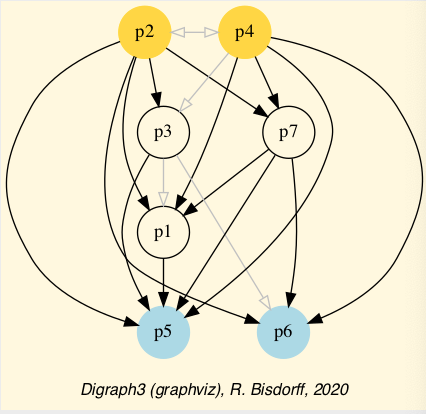
\includegraphics[height=6cm]{Figures/stdg.png}\hfill
  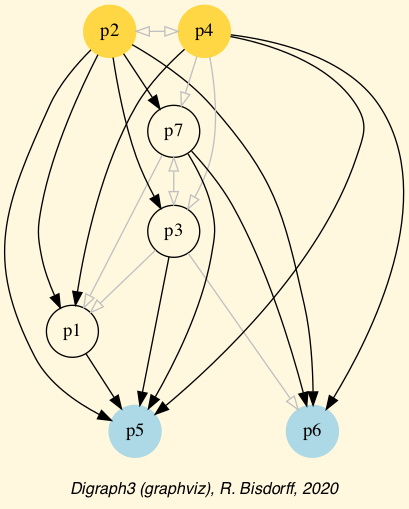
\includegraphics[height=6cm]{Figures/robg.png}
\caption{\emph{Standard} versus \emph{robust} strict outranking digraphs oriented by their initial and terminal prekernels} 
\label{fig:19.1}       % Give a unique label
\end{figure}
   
The robust version (right in Fig.~\ref{fig:19.1}) drops two strict outranking situations: between \texttt{p4} and \texttt{p7} and between \texttt{p7} and \texttt{p1}. The remaining 14 strict outranking (resp. outranked) situations are now all verified at a stability level of $+2$ and more (resp. $-2$ and less). They remain stably validated, hence, with all potential significance weights that are compatible with the given significance weights preordering (see Listing~\ref{list:19.2}).

To appreciate the apparent partial ordering of both the standard and the robust strict outranking digraphs shown in Fig.~\ref{fig:19.1}, let us have a final heat map view in Fig.~\ref{fig:19.2} on the underlying performance tableau ordered by the \NetFlows ranking rule actually applied to the robust version of the outranking digraph (see the \texttt{outrankingModel='this'} flag in Line 4 below).
\begin{lstlisting}[caption={Computing a robust performance heatmap view},label=list:19.9]
>>> rg.showHTMLPerformanceHeatmap(\
...           Correlations=True,\
...           colorLevels=5,\
...           outrankingModel='this',\
...           rankingRule='NetFlows')
\end{lstlisting}
\begin{figure}[h]
%\sidecaption
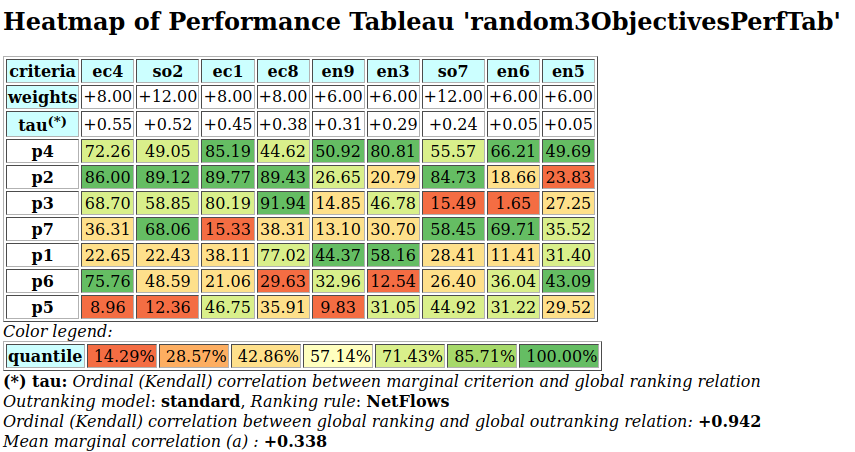
\includegraphics[width=12cm]{Figures/robustHeatmap.png}
\caption{Robust heatmap of the random 3 objectives performance tableau ordered by the \NetFlows ranking rule.} 
\label{fig:19.2}       % Give a unique label
\end{figure}
 As the inital prekernel \{\texttt{p2}, \texttt{p4}\} is in the robust outranking digraph validated at least at stability level $\pm 2$, recommending alternatives \texttt{p4}, as well as \texttt{p2}, as potential best choices, appears robustly justified. Alternative \texttt{p4} represents indeed an overall \emph{best compromise choice} between all decision objectives, whereas alternative \texttt{p2} gives an unanimous best choice with respect to two out of three decision objectives. Up to the decision maker to make his final choice.

\section{Characterising unopposed multiobjective outranking situations}
\label{sec:19.5}

When facing a performance tableau involving multiple decision objectives, the robustness level $\pm 3$  may lead to distinguishing what we call \emph{unopposed} outranking situations, like the one shown in the previous section between alternative \texttt{p4} and \texttt{p1} ($r(p4 \succsim p1) = +0.78$, see Listing \ref{list:19.4} Line 11), namely preferential situations that are more or less validated or invalidated by all the decision objectives.  
\begin{definition}[Unopposed outranking situation]\label{def:19.2}
\begin{itemize}
\item We say that decision alternative \texttt{x} \emph{unopposedly outranks} decision alternative \texttt{y} when  \texttt{x} positively outranks \texttt{y} on one or more decision objectives without \texttt{x} being positively outranked by \texttt{y} on any decision objective.
\item Dually, we say that decision alternative \texttt{x} \emph{is unopposedly outranked by} decision alternative \texttt{y} when \texttt{x} is positively outranked by \texttt{y} on one or more decision objectives without \texttt{x} positively outranking \texttt{y} on any decision objective.
\end{itemize}
\end{definition}

Let us reconsider, for instance, the performance tableau \texttt{pt} with three decision objectives already seen in Listing \ref{list:19.1}:
\begin{lstlisting}
>>> pt.showObjectives()
  *------ show objectives -------"
   Eco: Economical aspect
     ec1 criterion of objective Eco 8
     ec4 criterion of objective Eco 8
     ec8 criterion of objective Eco 8
    Total weight: 24.00 (3 criteria)
   Soc: Societal aspect
     so2 criterion of objective Soc 12
     so7 criterion of objective Soc 12
    Total weight: 24.00 (2 criteria)
   Env: Environmental aspect
     en3 criterion of objective Env 6
     en5 criterion of objective Env 6
     en6 criterion of objective Env 6
     en9 criterion of objective Env 6
    Total weight: 24.00 (4 criteria)
\end{lstlisting}
We notice in this example three decision objectives of equal importance (see Lines 3,13,17). What will be the outranking situations that are positively (resp.  negatively) validated for each one of the decision objectives taken individually ?

We may obtain such unopposed multiobjective outranking situations by operating an epistemic \emph{average fusion} (see the \texttt{symmetricAverage()} method \index{symmetricAverage@\texttt{symmetricAverage()}}) of the marginal outranking digraphs restricted to the coalition of criteria supporting each one of the decision objectives (see Listing \ref{list:19.9} below).
\begin{lstlisting}[caption={Computing unopposed outranking situations},label=list:19.9]
>>> from outrankingDigraphs import\
...                     BipolarOutrankingDigraph
>>> geco = BipolarOutrankingDigraph(pt,\
...                     objectivesSubset=['Eco'])
>>> gsoc = BipolarOutrankingDigraph(pt,\
...                     objectivesSubset=['Soc'])
>>> genv = BipolarOutrankingDigraph(pt,\
...                     objectivesSubset=['Env'])
>>> from digraphs import FusionLDigraph
>>> objectiveWeights = \
...               [pt.objectives[obj]['weight']\
...                      for obj in t.objectives] 
>>> uopg = FusionLDigraph([geco,gsoc,genv],\
...                   operator='o-average',\
...                   weights=objectiveWeights)
>>> uopg.showRelationTable(ReflexiveTerms=False)
  * ---- Relation Table -----
   r   |  'p1'   'p2'   'p3'   'p4'   'p5'   'p6'   'p7'   
  -----|------------------------------------------------
  'p1' |    -   +0.00  +0.00  -0.69  +0.39  +0.11  +0.00  
  'p2' | +0.00    -    +0.83  +0.00  +0.00  +0.00  +0.00  
  'p3' | +0.00  -0.33    -    +0.00  +0.50  +0.00  +0.00  
  'p4' | +0.78  +0.00  +0.61    -    +1.00  +1.00  +0.67  
  'p5' | -0.11  +0.00  +0.00  -0.89    -    +0.11  +0.00  
  'p6' | +0.00  +0.00  +0.00  -0.44  +0.17    -    +0.00  
  'p7' | +0.00  +0.00  +0.00  +0.00  +0.78  +0.42    -   
  Valuation domain: [-1.0; 1.0]
\end{lstlisting}
Positive (resp. negative) $r(x \succsim y)$ characteristic values, like $r(p1 \succsim p5) = +0.39$ (see Listing \ref{list:19.9} Line 20), show hence only outranking situations being validated (resp. invalidated) by one or more decision objectives without being invalidated (resp. validated) by any other decision objective.

For easily computing this kind of \emph{unopposed multiobjective} outranking digraphs, the \texttt{outrankingDigraphs} module conveniently provides a corresponding\\ \texttt{UnOpposedBipolarOutrankingDigraph} constructor \index{UnOpposedBipolarOutrankingDigraph@\texttt{UnOpposedBipolarOutrankingDigraph} class}.
\begin{lstlisting}[caption={Computing unopposed outranking digraphs},label=list:19.10]
>>> from outrankingDigraphs import\
...              UnOpposedBipolarOutrankingDigraph
>>> uopg = UnOpposedBipolarOutrankingDigraph(pt)
>>> uopg
  *------- Object instance description ------*
   Instance class      : UnOpposedBipolarOutrankingDigraph
   Instance name       : unopposed_outrankings
   Actions           : 7
   Criteria          : 9
   Size                : 13
   Oppositeness (%)    : 43.48
   Determinateness (%) : 61.71
   Valuation domain    : [-1.00;1.00]
   Attributes          : ['name', 'actions',
                'valuationdomain', 'objectives',
                'criteria', 'methodData',
                'evaluation', 'order', 'runTimes',
                'relation', ...
                'gamma', 'notGamma']
>>> uopg.computeOppositeness(InPercents=True)
  {'standardSize': 23, 'unopposedSize': 13,
   'oppositeness': 43.47826086956522}			   
\end{lstlisting}
The resulting \emph{unopposed} outranking digraph keeps in fact 13 (see Listing \ref{list:19.10} Lines 20-22) out of the 23 positively validated \emph{standard} outranking situations, leading to a degree of \emph{oppositeness} --preferential disagreement between decision objectives-- of $(1.0 - 13/23)\,=\,0.4348$.

We may now, for instance, verify the unopposed status of the outranking situation observed between alternatives \texttt{p1} and \texttt{p5}.
\begin{lstlisting}[caption={Example of unopposed multiobjective outranking situation},label=list:19.11]
>>> uopg.showPairwiseComparison('p1','p5')
 *------------  pairwise comparison ----*
  Comparing actions : ('p1', 'p5')
  crit. wght.  g(x)  g(y)    diff   | ind   pref     r()
  ec1   8.00  38.11  46.75  -8.64   | 5.00  10.00   +0.00
  ec4   8.00  22.65  8.96  +13.69   | 5.00  10.00   +8.00
  ec8   8.00  77.02  35.91  +41.11  | 5.00  10.00   +8.00
  en3   6.00  58.16  31.05  +27.11  | 5.00  10.00   +6.00
  en5   6.00  31.40  29.52  +1.88   | 5.00  10.00   +6.00
  en6   6.00  11.41  31.22  -19.81  | 5.00  10.00   -6.00
  en9   6.00  44.37  9.83  +34.54   | 5.00  10.00   +6.00
  so2   12.00  22.43  12.36  +10.07 | 5.00  10.00  +12.00
  so7   12.00  28.41  44.92  -16.51 | 5.00  10.00  -12.00
  Valuation in range: -72.00 to +72.00;           -------
                               global concordance: +28.00
\end{lstlisting}
In Listing \ref{list:19.11} we see that alternative \texttt{p1} does indeed positively outrank alternative \texttt{p5} from the economic perspective ($r(p1 \succsim_{Eco} p5) = +16/24$) as well as from the environmental perspective ($r(p1 \succsim_{Env} p5) = +12/24$). Whereas, from the societal perspective, both alternatives appear incomparable ($r(p1 \succsim_{Soc} p5) = 0/24$).

When proportionally equal criteria significance weights per objective are given, these outranking situations appear hence \emph{stable} with respect to all possible total importance weights we could allocate to the decision objectives.

This gives way for computing multiobjective \emph{Pareto efficient} choice recommendations. 

\section{Computing Pareto efficient multiobjective choices}
\label{sec:19.6}

Indeed, best choice recommendations, computed from an \emph{unopposed multiobjective} outranking digraph, deliver the case given \emph{Pareto efficient} choices. 
\begin{lstlisting}[caption={Pareto efficient multiobjective choice},label=list:19.12]
>>> uopg.showBestChoiceRecommendation()
  Best choice recommendation(s) (BCR)
   (in decreasing order of determinateness)   
   Credibility domain: [-1.00,1.00]
   === >> potential best choice(s)
   choice              : ['p2', 'p4', 'p7']
      independence        : 0.00
      dominance           : 0.33
      absorbency          : 0.00
      covering (%)        : 33.33
      determinateness (%) : 50.00
   === >> potential worst choice(s) 
   choice              : ['p3', 'p5', 'p6', 'p7']
      independence        : 0.00
      dominance           : -0.61
      absorbency          : 0.11
      covered (%)         : 33.33
      determinateness (%) : 50.00
\end{lstlisting}

Our previous \emph{robust} best choice recommendation (\texttt{p2} and \texttt{p4}, see Fig. \ref{fig:19.1}) remains, in this example here, \emph{stable}. We recover indeed the best choice recommendation [\texttt{p2}, \texttt{p4}, \texttt{p7}] (see Listing \ref{list:19.12} Line 6). Yet, notice that decision alternative \texttt{p7} appears to be at the same time a potential \emph{best} as well as a potential \emph{worst} choice recommendation (see Line 13), a consequence of \texttt{p7} being completely \emph{incomparable} to the other decision alternatives when restricting the comparability to only unopposed strict outranking situations. 

We may visualize this kind of Pareto efficient result in Fig. \ref{fig:19.3} below.
\begin{lstlisting}
>>> (~(-uopg)).exportGraphViz(fileName = 'unopDigraph',\
...                           bestChoice = ['p2','p4'],\
...                           worstChoice = ['p3','p5','p6'])
  *---- exporting a dot file for GraphViz tools ----*
   Exporting to unopDigraph.dot
   dot -Grankdir=BT -Tpng unopDigraph.dot -o unopDigraph.png
\end{lstlisting}
\begin{figure}[h]
%\sidecaption
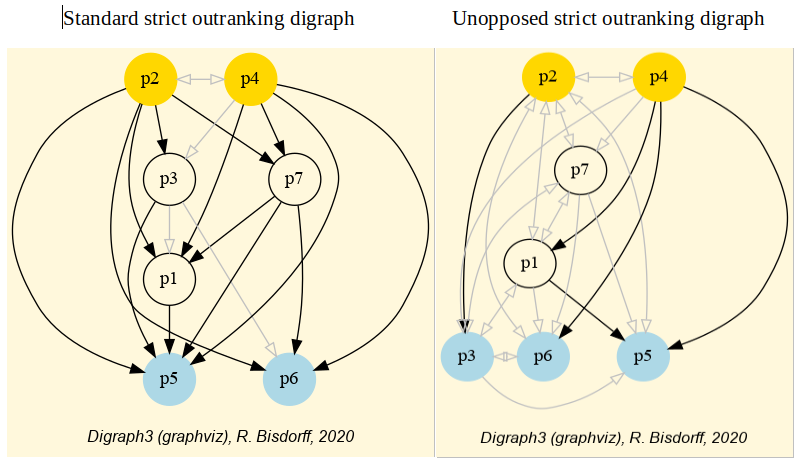
\includegraphics[width=12cm]{Figures/unopDigraph.png}
\caption{Standard versus \emph{unopposed} strict outranking digraphs oriented by best and worst choice recommendations.} 
\label{fig:19.3}       % Give a unique label
\end{figure}

In order to make now an eventual best unique choice, a decision maker will necessarily have to weight, in a second stage of the decision aiding process, the relative importance of the individual decision objectives.

\vspace{1cm}

For concluding, let us mention that it is precisely again our bipolar-valued logical characteristic framework that provides us here with a first order distributional dominance test for effectively qualifying the stability level $\pm 2$ robustness of an outranking digraph when facing performance tableaux with criteria of only ordinal-valued significances. A real world application of our stability analysis with such a kind of performance tableau may be consulted in \citep{BIS-2015}.
 
%%%%%%% The chapter bibliography
%\normallatexbib
\clearpage
%\phantomsection
%\addcontentsline{toc}{section}{Chapter Bibliography}
\bibliographystyle{spbasic}
%\typeout{}
\bibliography{03-backMatters/reference}
%\chapter[On robust outrankings]{Robustness analysis of outranking digraphs}
\label{sec:19}

\abstract*{ The required cardinal significance weights of the performance criteria represent the '\emph{Achilles}' heel of our outranking approach. Rarely will indeed a decision maker be cognitively competent for suggesting precise decimal-valued criteria significance weights. More often, the decision problem will involve more or less equally important decision objectives with more or less equi-significant criteria.
In this chapter, we study the stability of the outranking digraph when the criteria significance weights faithfully indicate solely an order of importance.}

\abstract{ The required cardinal significance weights of the performance criteria represent the '\emph{Achilles}' heel of our outranking approach. Rarely will indeed a decision maker be cognitively competent for suggesting precise decimal-valued criteria significance weights. More often, the decision problem will involve more or less equally important decision objectives with more or less equi-significant criteria.
In this chapter, we study the stability of the outranking digraph when the criteria significance weights faithfully indicate solely an order of importance.}

\section{Cardinal or ordinal criteria significance weights}
\label{sec:19.1}

A random example of such a decision problem with equally important decision objectives and equi-significant criteria may be generated with the \texttt{Random3\-Objectives\-PerformanceTableau} class \index{Random3ObjectivesPerformanceTableau@\texttt{Random3ObjectivesPerformanceTableau()}}.

\begin{lstlisting}[caption={Generate a Random 3 Objectives Performance Tableau},label=list:19.1]
>>> from randomPerfTabs import \
...           Random3ObjectivesPerformanceTableau
>>> pt = Random3ObjectivesPerformanceTableau(\
...           numberOfActions=7,\
...           numberOfCriteria=9,seed=102)
>>> pt
    *------- PerformanceTableau instance description ------*
    Instance class   : Random3ObjectivesPerformanceTableau
    Seed             : 102
    Instance name    : random3ObjectivesPerfTab
    Actions          : 7
    Objectives       : 3
    Criteria         : 9
    NA proportion (%): 0.0
    Attributes       : ['name', 'valueDigits', 'BigData',
              'OrdinalScales', 'missingDataProbability',
              'negativeWeightProbability', 'randomSeed',
              'sumWeights', 'valuationPrecision',
              'commonScale', 'objectiveSupportingTypes',
              'actions', 'objectives', 'criteriaWeightMode',
              'criteria', 'evaluation', 'weightPreorder']
>>> pt.showObjectives()
  *------ show objectives -------*
   Eco: Economical aspect
     ec1 criterion of objective Eco 8
     ec4 criterion of objective Eco 8
     ec8 criterion of objective Eco 8
     Total weight: 24.00 (3 criteria)
   Soc: Societal aspect
     so2 criterion of objective Soc 12
     so7 criterion of objective Soc 12
     Total weight: 24.00 (2 criteria)
   Env: Environmental aspect
     en3 criterion of objective Env 6
     en5 criterion of objective Env 6
     en6 criterion of objective Env 6
     en9 criterion of objective Env 6
     Total weight: 24.00 (4 criteria)
\end{lstlisting}
In Listing~\ref{list:19.1} one may notice a performance tableau \texttt{pt} describing seven decision alternatives that are assessed with respect to three equally important decision objectives concerning: --first, an \emph{economical} aspect (Line 24) with a coalition of three performance criteria of significance weight 8, --secondly, a \emph{societal} aspect (Line 29) with a coalition of two performance criteria of significance weight 12, and --thirdly, an \emph{environmental} aspect (Line 33) with a coalition four performance criteria of significance weight 6.

The question we tackle is the following: How \emph{dependent} on the actual values of the significance weights appears to be the corresponding bipolar-valued outranking digraph ? In the previous Chapter~\ref{sec:18} we assumed that the criteria significance weights were random variables. Here, we shall assume that we know for sure only the preordering of the significance weights. In our example we see indeed three increasing weight equivalence classes.
\begin{lstlisting}[caption={The significance weights preorder},label=list:19.2]
>>> pt.showWeightPreorder()
    ['en3', 'en5', 'en6', 'en9'] (6) <
    ['ec1', 'ec4', 'ec8'] (8) <
    ['so2', 'so7'] (12)
\end{lstlisting}
How stable appear now to be the outranking situations when allowing all possible significance weights that are compatible with this weights preorder shown in Listing~\ref{list:19.2} ?

\section{Qualifying the stability of outranking situations}
\label{sec:19.2}

Let us construct the bipolar-valued outranking digraph corresponding to the random 3-Objectives performance tableau \texttt{pt}.
\begin{lstlisting}[caption={Example Bipolar Outranking Digraph},label=list:19.3]
>>> from outrankingDigraphs import BipolarOutrankingDigraph
>>> g = BipolarOutrankingDigraph(pt)
>>> g.showRelationTable()
  * ---- Relation Table -----
   r(>=) |  'p1'   'p2'   'p3'   'p4'   'p5'   'p6'   'p7'   
   ------|------------------------------------------------
    'p1' | +1.00  -0.42  +0.00  -0.69  +0.39  +0.11  -0.06  
    'p2' | +0.58  +1.00  +0.83  +0.00  +0.58  +0.58  +0.58  
    'p3' | +0.25  -0.33  +1.00  +0.00  +0.50  +1.00  +0.25  
    'p4' | +0.78  +0.00  +0.61  +1.00  +1.00  +1.00  +0.67  
    'p5' | -0.11  -0.50  -0.25  -0.89  +1.00  +0.11  -0.14  
    'p6' | +0.22  -0.42  +0.00  -1.00  +0.17  +1.00  -0.11  
    'p7' | +0.22  -0.50  +0.17  -0.06  +0.78  +0.42  +1.00  
\end{lstlisting}
In Listing~\ref{list:19.3} Lines 7-13, we notice on the principal diagonal of the relation table the certainly validated reflexive terms $+1.00$ that are trivially independent of any significance weights. Now, we know for sure that \emph{unanimous} outranking situations are also completely independent of the significance weights. And, all outranking situations that are supported by a majority significance in each coalition of equi-significant criteria are as well independent of the actual importance we attach to each individual criteria coalition. We are furthermore able to effectively test if an outranking situation is in fact independent of all the potential significance weights that are compatible with the given preordering of the weights shown in Listing \ref{list:19.2} \citep{BIS-2014}. Mind that usually one also obtains outranking situations that are \emph{dependent} on the precise cardinal weights we allocate to the criteria significances.

Such a stability denotation of outranking situations may be inspected by using the \texttt{StabilityDenotation=True} flag \index{StabilityDenotation@\texttt{StabilityDenotation} flag} with the common \texttt{showRelationTable()} method.
\begin{lstlisting}[caption={Bipolar-valued outranking relation table with stability denotation},label=list:19.4]
>>> g.showRelationTable(StabilityDenotation=True)
  * ---- Relation Table -----
   r/(stab)  |  'p1'  'p2'  'p3'  'p4'  'p5'  'p6'  'p7'   
   ----------|------------------------------------------
     'p1'    | +1.00 -0.42 +0.00 -0.69 +0.39 +0.11 -0.06  
             |  (+4)  (-2)  (+0)  (-3)  (+2)  (+2)  (-1)  
     'p2'    | +0.58 +1.00 +0.83  0.00 +0.58 +0.58 +0.58  
             |  (+2)  (+4)  (+3)  (+2)  (+2)  (+2)  (+2)  
     'p3'    | +0.25 -0.33 +1.00  0.00 +0.50 +1.00 +0.25  
             |  (+2)  (-2)  (+4)   (0)  (+2)  (+2)  (+1)  
     'p4'    | +0.78  0.00 +0.61 +1.00 +1.00 +1.00 +0.67  
             |  (+3)  (-1)  (+3)  (+4)  (+4)  (+4)  (+2)  
     'p5'    | -0.11 -0.50 -0.25 -0.89 +1.00 +0.11 -0.14  
             |  (-2)  (-2)  (-2)  (-3)  (+4)  (+2)  (-2)  
     'p6'    | +0.22 -0.42  0.00 -1.00 +0.17 +1.00 -0.11
             |  (+2)  (-2)  (+1)  (-2)  (+2)  (+4)  (-2)  
     'p7'    | +0.22 -0.50 +0.17 -0.06 +0.78 +0.42 +1.00  
             |  (+2)  (-2)  (+1)  (-1)  (+3)  (+2)  (+4)  
\end{lstlisting}
In Listing~\ref{list:19.4} we may hence distinguish the following bipolar-valued stability levels:
\begin{itemize}[leftmargin=1cm]
\item [$\mathbf{\pm 4}$:] \emph{unanimous} outranking, resp. outranked situation. The pairwise trivial reflexive outrankings, for instance, all show this stability level;
\item [$\mathbf{\pm 3}$:] validated outranking, resp. outranked situation in \emph{each} coalition of equisignificant criteria. This is, for instance, the case for the outranking situation observed between alternatives \texttt{p1} and \texttt{p4} (see Listing \ref{list:19.4} Lines 6 and 12);
\item [$\mathbf{\pm 2}$:] validated outranking, resp. outranked situation with \emph{all} potential significance weights that are \emph{compatible} With the given significance preorder (see Listing \ref{list:19.2}). This is the case when comparing alternatives \texttt{p1} and \texttt{p2} (see Lines 6 and 8);
\item [$\mathbf{\pm 1}$:] validated outranking, resp. outranked situation with the \emph{precisely given decimal} significance weights, a situation we may observe between alternatives \texttt{p3} and \texttt{p7} (see Lines 10 and 16);
\item [$\mathbf{0}$:] \texttt{indeterminate} outranking situation, like the one between alternatives \texttt{p1} and \texttt{p3} (see Lines 6 and 10).
\end{itemize}

It is worthwhile noticing that, in the one limit case where all performance criteria appear equi-significant, i.e. there is given a single equivalence class containing all the criteria significance weights, one may only distinguish stability levels $\pm 4$ and $\pm 3$. In the other limit case, when all performance criteria admit different significanceweights, i.e. the significance weights may be linearly ordered without ties and no stability level $+3$ or $-3$ may be observed.

As mentioned above, all reflexive comparisons trivially confirm an unanimous outranking situation: all decision alternatives are indeed always``\emph{performing as well as}'' themselves. But there appear also two non reflexive unanimous outranking situations: when comparing, for instance, alternative \texttt{p4} with alternatives \texttt{p5} and \texttt{p6} (see Listing \ref{list:19.4} Lines 14 and 16). Let us inspect the details of how alternatives \texttt{p4} and \texttt{p5} compare.
\begin{lstlisting}
>>> g.showPairwiseComparison('p4','p5')
 *------------  pairwise comparison ----*
  Comparing actions : (p4, p5)
  crit. wght.  g(x)  g(y)    diff  | ind   pref    r()
  ec1   8.00  85.19  46.75  +38.44 | 5.00  10.00   +8.00
  ec4   8.00  72.26   8.96  +63.30 | 5.00  10.00   +8.00
  ec8   8.00  44.62  35.91   +8.71 | 5.00  10.00   +8.00
  en3   6.00  80.81  31.05  +49.76 | 5.00  10.00   +6.00
  en5   6.00  49.69  29.52  +20.17 | 5.00  10.00   +6.00
  en6   6.00  66.21  31.22  +34.99 | 5.00  10.00   +6.00
  en9   6.00  50.92   9.83  +41.09 | 5.00  10.00   +6.00
  so2  12.00  49.05  12.36  +36.69 | 5.00  10.00  +12.00
  so7  12.00  55.57  44.92  +10.65 | 5.00  10.00  +12.00
  Valuation in range: -72.00 to +72.00;          -------
                             global concordance:  +72.00
\end{lstlisting}
Alternative \texttt{p4} is indeed performing unanimously ``\emph{at least as well as}'' alternative \texttt{p5} and $r(p4 \succsim p5)\; =\; 72/72\; =\; +1.00$ (see Listing \ref{list:19.4} Line 11).

The converse comparison does not, however, deliver such an unanimous outranked situation. 
\begin{lstlisting}
>>> g.showPairwiseComparison('p5','p4')
 *------------  pairwise comparison ----*
  Comparing actions : (p5, p4)
  crit. wght.  g(x)  g(y)    diff  | ind   pref     r()
  ec1   8.00  46.75  85.19  -38.44 | 5.00  10.00   -8.00
  ec4   8.00   8.96  72.26  -63.30 | 5.00  10.00   -8.00
  ec8   8.00  35.91  44.62   -8.71 | 5.00  10.00   +0.00
  en3   6.00  31.05  80.81  -49.76 | 5.00  10.00   -6.00
  en5   6.00  29.52  49.69  -20.17 | 5.00  10.00   -6.00
  en6   6.00  31.22  66.21  -34.99 | 5.00  10.00   -6.00
  en9   6.00   9.83  50.92  -41.09 | 5.00  10.00   -6.00
  so2  12.00  12.36  49.05  -36.69 | 5.00  10.00  -12.00
  so7  12.00  44.92  55.57  -10.65 | 5.00  10.00  -12.00
  Valuation in range: -72.00 to +72.00;           ------
                             global concordance:  -64.00
\end{lstlisting}
The converse comparison only qualifies at stability level $-3$ (see Listing \ref{list:19.4} Line 13); $r(p5 \succsim p4)\; =\; -64/72\; =\; -0.89$). On criterion \texttt{ec8} we observe indeed a small negative performance difference of $-8.71$ (see Line 7 above) which is effectively below the supposed preference discrimination threshold of $10.00$. Yet, the outranked situation is supported by a majority of criteria in each decision objective. Hence, the reported preferential situation is completely independent of any chosen significance weights.

Let us now consider a comparison, like the one between alternatives \texttt{p2} and \texttt{p1}, that is qualified at stability level $+2$, resp. $-2$.
\begin{lstlisting}[caption={Comparison of alternatives \texttt{p2} and \texttt{p1}},label=list:19.5]
>>> g.showPairwiseOutrankings('p2','p1')
  *------------  pairwise comparison ----*
   Comparing actions : (p2, p1)
   crit. wght.  g(x)  g(y)    diff  | ind   pref     r()
   ec1   8.00  89.77  38.11  +51.66 | 5.00  10.00   +8.00
   ec4   8.00  86.00  22.65  +63.35 | 5.00  10.00   +8.00
   ec8   8.00  89.43  77.02  +12.41 | 5.00  10.00   +8.00
   en3   6.00  20.79  58.16  -37.37 | 5.00  10.00   -6.00
   en5   6.00  23.83  31.40   -7.57 | 5.00  10.00   +0.00
   en6   6.00  18.66  11.41   +7.25 | 5.00  10.00   +6.00
   en9   6.00  26.65  44.37  -17.72 | 5.00  10.00   -6.00
   so2  12.00  89.12  22.43  +66.69 | 5.00  10.00  +12.00
   so7  12.00  84.73  28.41  +56.32 | 5.00  10.00  +12.00
   Valuation in range: -72.00 to +72.00;          -------
                              global concordance:  +42.00
    *------------  pairwise comparison ----*
    Comparing actions : ('p1', 'p2')
    crit. wght.  g(x)  g(y)    diff  | ind   pref     r()
    ec1   8.00  38.11  89.77  -51.66 | 5.00  10.00   -8.00
    ec4   8.00  22.65  86.00  -63.35 | 5.00  10.00   -8.00
    ec8   8.00  77.02  89.43  -12.41 | 5.00  10.00   -8.00
    en3   6.00  58.16  20.79  +37.37 | 5.00  10.00   +6.00
    en5   6.00  31.40  23.83   +7.57 | 5.00  10.00   +6.00 
    en6   6.00  11.41  18.66   -7.25 | 5.00  10.00   +0.00
    en9   6.00  44.37  26.65  +17.72 | 5.00  10.00   +6.00
    so2  12.00  22.43  89.12  -66.69 | 5.00  10.00  -12.00
    so7  12.00  28.41  84.73  -56.32 | 5.00  10.00  -12.00
    Valuation in range: -72.00 to +72.00;          -------
                                global concordance: -30.00
\end{lstlisting}
In both comparisons, the performances observed with respect to the environmental decision objective are not validating with a significant majority the outranking, resp. outranked situation. Hence, the stability of the reported preferential situations is in fact dependent on choosing significance weights that are compatible with the given significance weights preorder (see Listing \ref{list:19.2}).

Let us finally inspect a comparison that is only qualified at stability level $+1$, like the one between alternatives \texttt{p7} and \texttt{p3}.
\begin{lstlisting}[caption={Comparison of alternatives \texttt{p7} and \texttt{p3}},label=list:19.6]
>>> g.showPairwiseOutrankings('p7','p3')
 *------------  pairwise comparison ----*
  Comparing actions : ('p7', 'p3')
  crit. wght.  g(x)  g(y)    diff  | ind   pref     r()
  ec1   8.00  15.33  80.19  -64.86 | 5.00  10.00   -8.00
  ec4   8.00  36.31  68.70  -32.39 | 5.00  10.00   -8.00
  ec8   8.00  38.31  91.94  -53.63 | 5.00  10.00   -8.00
  en3   6.00  30.70  46.78  -16.08 | 5.00  10.00   -6.00
  en5   6.00  35.52  27.25   +8.27 | 5.00  10.00   +6.00
  en6   6.00  69.71   1.65  +68.06 | 5.00  10.00   +6.00
  en9   6.00  13.10  14.85   -1.75 | 5.00  10.00   +6.00
  so2  12.00  68.06  58.85   +9.21 | 5.00  10.00  +12.00
  so7  12.00  58.45  15.49  +42.96 | 5.00  10.00  +12.00
  Valuation in range: -72.00 to +72.00;          -------
                              global concordance: +12.00
 *------------  pairwise comparison ----*
  Comparing actions : ('p3', 'p7')
  crit. wght.  g(x)  g(y)    diff  | ind   pref     r()
  ec1   8.00  80.19  15.33  +64.86 | 5.00  10.00   +8.00
  ec4   8.00  68.70  36.31  +32.39 | 5.00  10.00   +8.00
  ec8   8.00  91.94  38.31  +53.63 | 5.00  10.00   +8.00
  en3   6.00  46.78  30.70  +16.08 | 5.00  10.00   +6.00
  en5   6.00  27.25  35.52   -8.27 | 5.00  10.00   +0.00
  en6   6.00   1.65  69.71  -68.06 | 5.00  10.00   -6.00
  en9   6.00  14.85  13.10   +1.75 | 5.00  10.00   +6.00
  so2  12.00  58.85  68.06   -9.21 | 5.00  10.00   +0.00
  so7  12.00  15.49  58.45  -42.96 | 5.00  10.00  -12.00
  Valuation in range: -72.00 to +72.00;          -------
                              global concordance: +18.00
\end{lstlisting}
In both cases, choosing only significances that are compatible with the given weights preorder will not always result in positively validated outranking situations.

\section{Computing the stability denotation of outranking situations}
\label{sec:19.3}

Stability levels $\pm 4$ and $\pm 3$ are, the case given, easy to detect. Detecting a stability level $\pm 2$ is far less obvious.  Now, it is precisely again the bipolar-valued epistemic characteristic domain that will give us a way to implement an effective test for stability level $+2$ and $-2$ \citep{BIS-2004b,BIS-2004c}. 

Let us consider the significance equivalence classes we observe in the given weights preorder. Here we observe three weight classes: $6$, $8$, and $12$, in increasing order (see Listing \ref{list:19.2}). In the pairwise comparisons, shown above, these equivalence classes may appear positively or negatively, besides the indeterminate significance of value $0.00$. We thus get the following ordered bipolar list of significance weights: $W = [-12. -8. -6, 0, 6, 8, 12]$.

In all the pairwise marginal comparisons shown in the previous Section, we may observe that each one of the nine criteria assigns one precise item out of this list $W$. Let us denote $q[i]$ the number of criteria assigning item $W[i]$, and $Q[i]$ the cumulative sums of these $q[i]$ counts, where $i$ is an index in the range of the length of list $W$.

In the comparison of alternatives \texttt{p2} and \texttt{p1}, for instance (see Listing \ref{list:19.5}), we observe the following counts: \hfill
\begin{center}
\begin{tabular}{l|r|r|r|r|r|r|r}
 \svhline\noalign{\smallskip}
  $W[i]$ & -12 & -8  & -6  &  0  &  6  &  8 &  12\\  
 \noalign{\smallskip}\hline\noalign{\smallskip}
$q[i]$  &  0 &  0 &   2 &   1  &  1  &  3  &  2 \\
$Q[i]$  &  0 &  0 &   2 &   3  &  4  &  7  &  9 \\
      \noalign{\smallskip}\hline
\end{tabular}
\end{center}

\noindent Let use denote $-q$ and $-Q$ the reversed versions of the $q$ and the $Q$ lists. We thus obtain the following result.\hfill
\begin{center}
\begin{tabular}{l|r|r|r|r|r|r|r}
 \svhline\noalign{\smallskip}
  $W[i]$ & -12 & -8  & -6  &  0  &  6  &  8 &  12\\  
 \noalign{\smallskip}\hline\noalign{\smallskip}
  $-q[i]$  &  2 &  3 &   1 &   1  &  2  &  0  &  0 \\
  $-Q[i]$  &  2 &  5 &   6 &   7  &  9  &  9  &  9 \\
 \noalign{\smallskip}\hline
\end{tabular}
\end{center}

Now, a pairwise outranking situation will be qualified at stability level $+2$, i.e. positively validated with any significance weights that are compatible with the given weights preorder, when for all $i$, we observe $Q[i] \leq -Q[i]$ and there exists one $i$ such that $Q[i] < -Q[i]$. Similarly, a pairwise outranked situation will be qualified at stability level $-2$, when for all $i$, we observe $Q[i] \geq -Q[i]$ and there exists one $i$ such that $Q[i] > -Q[i]$ \citep{BIS-2004c}.

We may verify, for instance, that the outranking situation observed between alternatives \texttt{p2} and \texttt{p1} does indeed verify this \emph{first order distributional dominance} condition. \hfill
\begin{center}
\begin{tabular}{l|r|r|r|r|r|r|r}
 \svhline\noalign{\smallskip}
  $W[i]$ & -12 & -8  & -6  &  0  &  6  &  8 &  12\\  
 \noalign{\smallskip}\hline\noalign{\smallskip}
  $Q[i]$  &  0 &  0 &   2 &   3  &  4  &  7  &  9 \\
  $-Q[i]$  &  2 &  5 &   6 &   7  &  9  &  9  &  9 \\
 \noalign{\smallskip}\hline
\end{tabular}
\end{center}

Notice that outranking situations qualified at stability levels $\pm 4$ and $\pm 3$, evidently also verify the stability level $\pm 2$ test above. The outranking situation between alternatives \texttt{p7} and \texttt{p3} does not, however, verify this test (see Listing \ref{list:19.6}).\hfill
\begin{center}
\begin{tabular}{l|r|r|r|r|r|r|r}
 \svhline\noalign{\smallskip}
  $W[i]$ & -12 & -8  & -6  &  0  &  6  &  8 &  12\\  
 \noalign{\smallskip}\hline\noalign{\smallskip}
  $q[i]$  &  0 &  3 &   1 &   0  &  3  &  0  &  2 \\
  $Q[i]$  &  0 &  3 &   4 &   4  &  7  &  7  &  9 \\
  $-Q[i]$  &  2 &  2 &   5 &   5  &  6  &  9  &  9 \\
 \noalign{\smallskip}\hline
\end{tabular}
\end{center}
This time, not all the $Q[i]$ are \emph{lower or equal} than the corresponding $-Q[i]$ terms. Hence the outranking situation between \texttt{p7} and \texttt{p3} is not positively validated with all potential significance weights that are compatible with the given weights preorder.

Using this stability denotation, we may, hence, define the following \emph{robust} version of a bipolar-valued outranking digraph.

\section{Robust bipolar-valued outranking digraphs}
\label{sec:19.4}

\begin{definition}[Robust outranking situation]\label{def:19.1}
\begin{itemize}
\item We say that decision alternative \texttt{x} \emph{robustly outranks} decision alternative \texttt{y} when:
\begin{itemize}[nosep]
\item \texttt{x} positively outranks \texttt{y} at stability level $+2$ or higher and
\item we may not observe any considerable counter-performance of \texttt{x} on a discordant criterion.
\end{itemize}
\item Dually, we say that decision alternative \texttt{x} \emph{does not robustly outrank} decision alternative \texttt{y} when:
\begin{itemize}[nosep]
\item \texttt{x} is positively outranked by \texttt{y} at stability level $-2$ or lower and
\item we may not observe any considerable better performance of \texttt{x} on a discordant criterion.
\end{itemize}
\item Otherwise the outranking situation is indeterminate.
\end{itemize}
\end{definition}
The corresponding \emph{robust} outranking digraph may be computed as follows with the \texttt{RobustOutrankingDigraph} class\index{RobustOutrankingDigraph@\texttt{RobustOutrankingDigraph} class}:
\begin{lstlisting}[caption={Computing a robust outranking digraph},label=list:19.7]
>>> from outrankingDigraphs import\
...              RobustOutrankingDigraph
>>> rg = RobustOutrankingDigraph(pt) # same t as before
>>> rg
  *------- Object instance description ------*
   Instance class      : RobustOutrankingDigraph
   Instance name       : robust_random3ObjectivesPerfTab
   Actions             : 7
   Criteria            : 9
   Size                : 22
   Determinateness (%) : 68.45
   Valuation domain    : [-1.00;1.00]
   Attributes          : ['name', 'methodData', 'actions',
         'order', 'criteria', 'evaluation',
         'vetos', 'valuationdomain',
         'cardinalRelation', 'ordinalRelation',
         'equisignificantRelation', 'unanimousRelation',
         'relation', 'gamma', 'notGamma']
>>> rg.showRelationTable()
  * ---- Relation Table -----
   r/(stab) |  'p1'  'p2'  'p3'  'p4'  'p5'  'p6'  'p7'   
   ---------|------------------------------------------
     'p1'   | +1.00 -0.42 +0.00 -0.69 +0.39 +0.11 +0.00  
            |  (+4)  (-2)  (+0)  (-3)  (+2)  (+2)  (-1)  
     'p2'   | +0.58 +1.00 +0.83 +0.00 +0.58 +0.58 +0.58  
            |  (+2)  (+4)  (+3)  (+2)  (+2)  (+2)  (+2)  
     'p3'   | +0.25 -0.33 +1.00 +0.00 +0.50 +1.00 +0.00  
            |  (+2)  (-2)  (+4)  (+0)  (+2)  (+2)  (+1)  
     'p4'   | +0.78 +0.00 +0.61 +1.00 +1.00 +1.00 +0.67  
            |  (+3)  (-1)  (+3)  (+4)  (+4)  (+4)  (+2)  
     'p5'   | -0.11 -0.50 -0.25 -0.89 +1.00 +0.11 -0.14  
            |  (-2)  (-2)  (-2)  (-3)  (+4)  (+2)  (-2)  
     'p6'   | +0.22 -0.42 +0.00 -1.00 +0.17 +1.00 -0.11  
            |  (+2)  (-2)  (+1)  (-2)  (+2)  (+4)  (-2)  
     'p7'   | +0.22 -0.50 +0.00 +0.00 +0.78 +0.42 +1.00  
            |  (+2)  (-2)  (+1)  (-1)  (+3)  (+2)  (+4)  
\end{lstlisting}
We may notice that all outranking situations, qualified at stability level $\pm 1$, are now put to an \emph{indeterminate} status. In the example here, three positive outrankings get dropped: between \texttt{p3} and \texttt{p7}, between \texttt{p7} and \texttt{p3}, and between \texttt{p6} and \texttt{p3}, where the last situation is actually already doubtful because of a veto situation (see Listing \ref{list:19.7} Lines 22-35). Three negative outrankings get dropped as well: between \texttt{p1} and \texttt{p7}, between \texttt{p4} and \texttt{p2}, and between \texttt{p7} and \texttt{p4} (see Lines 22-35).

Notice by the way that outranking or outranked situations, although qualified at level $\pm 2$ or $\pm 3$ may nevertheless become doubtful because of considerable performance differences. We may observe such a doubtful situation when comparing, for instance, alternatives \texttt{p2} and \texttt{p4} (see Listing \ref{list:19.7} Lines 24-25).
\begin{lstlisting}[caption={Comparing alternatives \texttt{p2} and \texttt{p4}},label=list:19.8,basicstyle=\ttfamily\scriptsize]
>>> rg.showPairwiseComparison('p2','p4')
   *------------  pairwise comparison ----*
    Comparing actions : (p2, p4)
    crit. wght.  g(x)  g(y)    diff  	| ind   pref    r() 	|   v    veto
    -------------------------------------------------------------------------
    ec1   8.00  89.77  85.19  +4.58 	| 5.00  10.00   +8.00 	| 
    ec4   8.00  86.00  72.26  +13.74 	| 5.00  10.00   +8.00 	| 
    ec8   8.00  89.43  44.62  +44.81 	| 5.00  10.00   +8.00 	| 
    en3   6.00  20.79  80.81  -60.02 	| 5.00  10.00   -6.00 	| 60.00 -1.00
    en5   6.00  23.83  49.69  -25.86 	| 5.00  10.00   -6.00 	| 
    en6   6.00  18.66  66.21  -47.55 	| 5.00  10.00   -6.00 	| 
    en9   6.00  26.65  50.92  -24.27 	| 5.00  10.00   -6.00 	| 
    so2   12.00  89.12  49.05  +40.07 	| 5.00  10.00  +12.00 	| 
    so7   12.00  84.73  55.57  +29.16 	| 5.00  10.00  +12.00   |
    Valuation in range: -72.00 to +72.00;             -------
                                   global concordance: +24.00      
\end{lstlisting}
Despite being robust, the apparent positive outranking situation between alternatives \texttt{p2} and \texttt{p4} becomes doubtful because of a considerable counter-performance ($-60.02$) of \texttt{p2} observed on criterion \texttt{en3}, a negative difference which exceeds slightly the assumed veto discrimination threshold $v = 60.00$ (see Listing \ref{list:19.8} Line 9).

We may finally compare in Fig. \ref{fig:19.1} the \emph{standard} and the \emph{robust} version of the corresponding strict outranking digraphs, both oriented by their respective identical initial and terminal prekernels.
\begin{lstlisting}
>>> rg.showPreKernels()
  *--- Computing preKernels ---*
   Dominant preKernels :
   ['p2', 'p4']
    independence :  0.00
    dominance    :  0.667
    absorbency   :  -0.50
    covering     :  1.000
   Absorbent preKernels :
   ['p5']
    independence :  1.0
    dominance    :  -0.889
    absorbency   :  0.167
    covered      :  1.000
   ['p6']
    independence :  1.0
    dominance    :  -1.0
    absorbency   :  0.111
    covered      :  1.000
\end{lstlisting}
\begin{figure}[h]
  % \sidecaption
  Standard strict outranking digraph \hfill Robust strict outranking digraph \\
  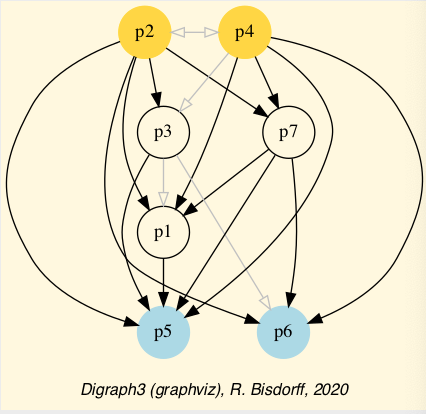
\includegraphics[height=6cm]{Figures/stdg.png}\hfill
  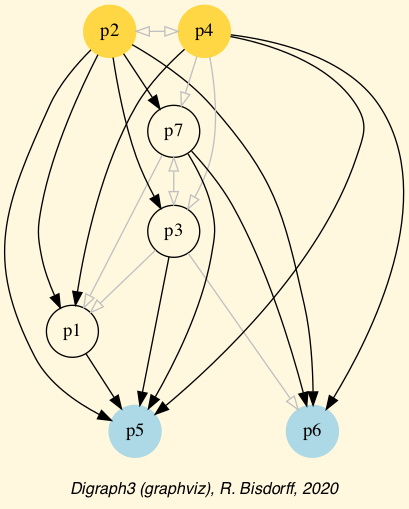
\includegraphics[height=6cm]{Figures/robg.png}
\caption{\emph{Standard} versus \emph{robust} strict outranking digraphs oriented by their initial and terminal prekernels} 
\label{fig:19.1}       % Give a unique label
\end{figure}
   
The robust version (right in Fig.~\ref{fig:19.1}) drops two strict outranking situations: between \texttt{p4} and \texttt{p7} and between \texttt{p7} and \texttt{p1}. The remaining 14 strict outranking (resp. outranked) situations are now all verified at a stability level of $+2$ and more (resp. $-2$ and less). They remain stably validated, hence, with all potential significance weights that are compatible with the given significance weights preordering (see Listing~\ref{list:19.2}).

To appreciate the apparent partial ordering of both the standard and the robust strict outranking digraphs shown in Fig.~\ref{fig:19.1}, let us have a final heat map view in Fig.~\ref{fig:19.2} on the underlying performance tableau ordered by the \NetFlows ranking rule actually applied to the robust version of the outranking digraph (see the \texttt{outrankingModel='this'} flag in Line 4 below).
\begin{lstlisting}[caption={Computing a robust performance heatmap view},label=list:19.9]
>>> rg.showHTMLPerformanceHeatmap(\
...           Correlations=True,\
...           colorLevels=5,\
...           outrankingModel='this',\
...           rankingRule='NetFlows')
\end{lstlisting}
\begin{figure}[h]
%\sidecaption
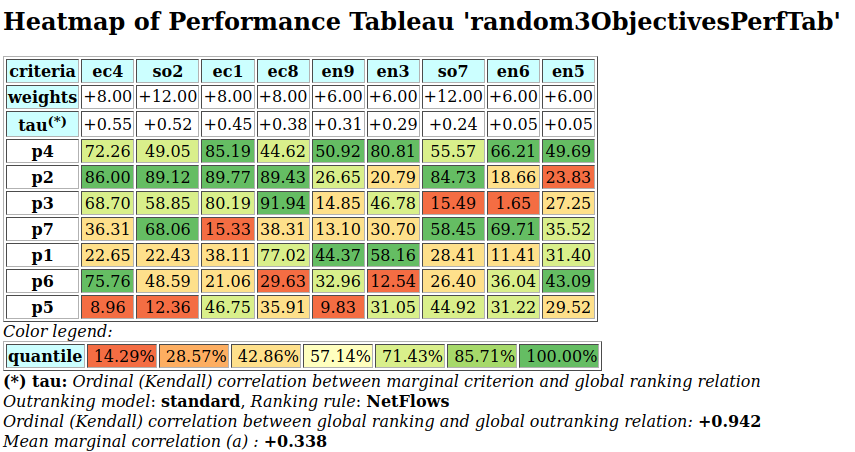
\includegraphics[width=12cm]{Figures/robustHeatmap.png}
\caption{Robust heatmap of the random 3 objectives performance tableau ordered by the \NetFlows ranking rule.} 
\label{fig:19.2}       % Give a unique label
\end{figure}
 As the inital prekernel \{\texttt{p2}, \texttt{p4}\} is in the robust outranking digraph validated at least at stability level $\pm 2$, recommending alternatives \texttt{p4}, as well as \texttt{p2}, as potential best choices, appears robustly justified. Alternative \texttt{p4} represents indeed an overall \emph{best compromise choice} between all decision objectives, whereas alternative \texttt{p2} gives an unanimous best choice with respect to two out of three decision objectives. Up to the decision maker to make his final choice.

\section{Characterising unopposed multiobjective outranking situations}
\label{sec:19.5}

When facing a performance tableau involving multiple decision objectives, the robustness level $\pm 3$  may lead to distinguishing what we call \emph{unopposed} outranking situations, like the one shown in the previous section between alternative \texttt{p4} and \texttt{p1} ($r(p4 \succsim p1) = +0.78$, see Listing \ref{list:19.4} Line 11), namely preferential situations that are more or less validated or invalidated by all the decision objectives.  
\begin{definition}[Unopposed outranking situation]\label{def:19.2}
\begin{itemize}
\item We say that decision alternative \texttt{x} \emph{unopposedly outranks} decision alternative \texttt{y} when  \texttt{x} positively outranks \texttt{y} on one or more decision objectives without \texttt{x} being positively outranked by \texttt{y} on any decision objective.
\item Dually, we say that decision alternative \texttt{x} \emph{is unopposedly outranked by} decision alternative \texttt{y} when \texttt{x} is positively outranked by \texttt{y} on one or more decision objectives without \texttt{x} positively outranking \texttt{y} on any decision objective.
\end{itemize}
\end{definition}

Let us reconsider, for instance, the performance tableau \texttt{pt} with three decision objectives already seen in Listing \ref{list:19.1}:
\begin{lstlisting}
>>> pt.showObjectives()
  *------ show objectives -------"
   Eco: Economical aspect
     ec1 criterion of objective Eco 8
     ec4 criterion of objective Eco 8
     ec8 criterion of objective Eco 8
    Total weight: 24.00 (3 criteria)
   Soc: Societal aspect
     so2 criterion of objective Soc 12
     so7 criterion of objective Soc 12
    Total weight: 24.00 (2 criteria)
   Env: Environmental aspect
     en3 criterion of objective Env 6
     en5 criterion of objective Env 6
     en6 criterion of objective Env 6
     en9 criterion of objective Env 6
    Total weight: 24.00 (4 criteria)
\end{lstlisting}
We notice in this example three decision objectives of equal importance (see Lines 3,13,17). What will be the outranking situations that are positively (resp.  negatively) validated for each one of the decision objectives taken individually ?

We may obtain such unopposed multiobjective outranking situations by operating an epistemic \emph{average fusion} (see the \texttt{symmetricAverage()} method \index{symmetricAverage@\texttt{symmetricAverage()}}) of the marginal outranking digraphs restricted to the coalition of criteria supporting each one of the decision objectives (see Listing \ref{list:19.9} below).
\begin{lstlisting}[caption={Computing unopposed outranking situations},label=list:19.9]
>>> from outrankingDigraphs import\
...                     BipolarOutrankingDigraph
>>> geco = BipolarOutrankingDigraph(pt,\
...                     objectivesSubset=['Eco'])
>>> gsoc = BipolarOutrankingDigraph(pt,\
...                     objectivesSubset=['Soc'])
>>> genv = BipolarOutrankingDigraph(pt,\
...                     objectivesSubset=['Env'])
>>> from digraphs import FusionLDigraph
>>> objectiveWeights = \
...               [pt.objectives[obj]['weight']\
...                      for obj in t.objectives] 
>>> uopg = FusionLDigraph([geco,gsoc,genv],\
...                   operator='o-average',\
...                   weights=objectiveWeights)
>>> uopg.showRelationTable(ReflexiveTerms=False)
  * ---- Relation Table -----
   r   |  'p1'   'p2'   'p3'   'p4'   'p5'   'p6'   'p7'   
  -----|------------------------------------------------
  'p1' |    -   +0.00  +0.00  -0.69  +0.39  +0.11  +0.00  
  'p2' | +0.00    -    +0.83  +0.00  +0.00  +0.00  +0.00  
  'p3' | +0.00  -0.33    -    +0.00  +0.50  +0.00  +0.00  
  'p4' | +0.78  +0.00  +0.61    -    +1.00  +1.00  +0.67  
  'p5' | -0.11  +0.00  +0.00  -0.89    -    +0.11  +0.00  
  'p6' | +0.00  +0.00  +0.00  -0.44  +0.17    -    +0.00  
  'p7' | +0.00  +0.00  +0.00  +0.00  +0.78  +0.42    -   
  Valuation domain: [-1.0; 1.0]
\end{lstlisting}
Positive (resp. negative) $r(x \succsim y)$ characteristic values, like $r(p1 \succsim p5) = +0.39$ (see Listing \ref{list:19.9} Line 20), show hence only outranking situations being validated (resp. invalidated) by one or more decision objectives without being invalidated (resp. validated) by any other decision objective.

For easily computing this kind of \emph{unopposed multiobjective} outranking digraphs, the \texttt{outrankingDigraphs} module conveniently provides a corresponding\\ \texttt{UnOpposedBipolarOutrankingDigraph} constructor \index{UnOpposedBipolarOutrankingDigraph@\texttt{UnOpposedBipolarOutrankingDigraph} class}.
\begin{lstlisting}[caption={Computing unopposed outranking digraphs},label=list:19.10]
>>> from outrankingDigraphs import\
...              UnOpposedBipolarOutrankingDigraph
>>> uopg = UnOpposedBipolarOutrankingDigraph(pt)
>>> uopg
  *------- Object instance description ------*
   Instance class      : UnOpposedBipolarOutrankingDigraph
   Instance name       : unopposed_outrankings
   Actions           : 7
   Criteria          : 9
   Size                : 13
   Oppositeness (%)    : 43.48
   Determinateness (%) : 61.71
   Valuation domain    : [-1.00;1.00]
   Attributes          : ['name', 'actions',
                'valuationdomain', 'objectives',
                'criteria', 'methodData',
                'evaluation', 'order', 'runTimes',
                'relation', ...
                'gamma', 'notGamma']
>>> uopg.computeOppositeness(InPercents=True)
  {'standardSize': 23, 'unopposedSize': 13,
   'oppositeness': 43.47826086956522}			   
\end{lstlisting}
The resulting \emph{unopposed} outranking digraph keeps in fact 13 (see Listing \ref{list:19.10} Lines 20-22) out of the 23 positively validated \emph{standard} outranking situations, leading to a degree of \emph{oppositeness} --preferential disagreement between decision objectives-- of $(1.0 - 13/23)\,=\,0.4348$.

We may now, for instance, verify the unopposed status of the outranking situation observed between alternatives \texttt{p1} and \texttt{p5}.
\begin{lstlisting}[caption={Example of unopposed multiobjective outranking situation},label=list:19.11]
>>> uopg.showPairwiseComparison('p1','p5')
 *------------  pairwise comparison ----*
  Comparing actions : ('p1', 'p5')
  crit. wght.  g(x)  g(y)    diff   | ind   pref     r()
  ec1   8.00  38.11  46.75  -8.64   | 5.00  10.00   +0.00
  ec4   8.00  22.65  8.96  +13.69   | 5.00  10.00   +8.00
  ec8   8.00  77.02  35.91  +41.11  | 5.00  10.00   +8.00
  en3   6.00  58.16  31.05  +27.11  | 5.00  10.00   +6.00
  en5   6.00  31.40  29.52  +1.88   | 5.00  10.00   +6.00
  en6   6.00  11.41  31.22  -19.81  | 5.00  10.00   -6.00
  en9   6.00  44.37  9.83  +34.54   | 5.00  10.00   +6.00
  so2   12.00  22.43  12.36  +10.07 | 5.00  10.00  +12.00
  so7   12.00  28.41  44.92  -16.51 | 5.00  10.00  -12.00
  Valuation in range: -72.00 to +72.00;           -------
                               global concordance: +28.00
\end{lstlisting}
In Listing \ref{list:19.11} we see that alternative \texttt{p1} does indeed positively outrank alternative \texttt{p5} from the economic perspective ($r(p1 \succsim_{Eco} p5) = +16/24$) as well as from the environmental perspective ($r(p1 \succsim_{Env} p5) = +12/24$). Whereas, from the societal perspective, both alternatives appear incomparable ($r(p1 \succsim_{Soc} p5) = 0/24$).

When proportionally equal criteria significance weights per objective are given, these outranking situations appear hence \emph{stable} with respect to all possible total importance weights we could allocate to the decision objectives.

This gives way for computing multiobjective \emph{Pareto efficient} choice recommendations. 

\section{Computing Pareto efficient multiobjective choices}
\label{sec:19.6}

Indeed, best choice recommendations, computed from an \emph{unopposed multiobjective} outranking digraph, deliver the case given \emph{Pareto efficient} choices. 
\begin{lstlisting}[caption={Pareto efficient multiobjective choice},label=list:19.12]
>>> uopg.showBestChoiceRecommendation()
  Best choice recommendation(s) (BCR)
   (in decreasing order of determinateness)   
   Credibility domain: [-1.00,1.00]
   === >> potential best choice(s)
   choice              : ['p2', 'p4', 'p7']
      independence        : 0.00
      dominance           : 0.33
      absorbency          : 0.00
      covering (%)        : 33.33
      determinateness (%) : 50.00
   === >> potential worst choice(s) 
   choice              : ['p3', 'p5', 'p6', 'p7']
      independence        : 0.00
      dominance           : -0.61
      absorbency          : 0.11
      covered (%)         : 33.33
      determinateness (%) : 50.00
\end{lstlisting}

Our previous \emph{robust} best choice recommendation (\texttt{p2} and \texttt{p4}, see Fig. \ref{fig:19.1}) remains, in this example here, \emph{stable}. We recover indeed the best choice recommendation [\texttt{p2}, \texttt{p4}, \texttt{p7}] (see Listing \ref{list:19.12} Line 6). Yet, notice that decision alternative \texttt{p7} appears to be at the same time a potential \emph{best} as well as a potential \emph{worst} choice recommendation (see Line 13), a consequence of \texttt{p7} being completely \emph{incomparable} to the other decision alternatives when restricting the comparability to only unopposed strict outranking situations. 

We may visualize this kind of Pareto efficient result in Fig. \ref{fig:19.3} below.
\begin{lstlisting}
>>> (~(-uopg)).exportGraphViz(fileName = 'unopDigraph',\
...                           bestChoice = ['p2','p4'],\
...                           worstChoice = ['p3','p5','p6'])
  *---- exporting a dot file for GraphViz tools ----*
   Exporting to unopDigraph.dot
   dot -Grankdir=BT -Tpng unopDigraph.dot -o unopDigraph.png
\end{lstlisting}
\begin{figure}[h]
%\sidecaption
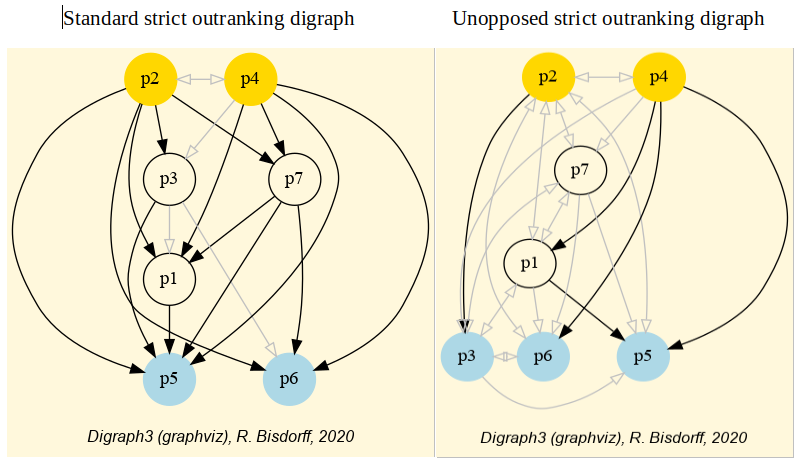
\includegraphics[width=12cm]{Figures/unopDigraph.png}
\caption{Standard versus \emph{unopposed} strict outranking digraphs oriented by best and worst choice recommendations.} 
\label{fig:19.3}       % Give a unique label
\end{figure}

In order to make now an eventual best unique choice, a decision maker will necessarily have to weight, in a second stage of the decision aiding process, the relative importance of the individual decision objectives.

\vspace{1cm}

For concluding, let us mention that it is precisely again our bipolar-valued logical characteristic framework that provides us here with a first order distributional dominance test for effectively qualifying the stability level $\pm 2$ robustness of an outranking digraph when facing performance tableaux with criteria of only ordinal-valued significances. A real world application of our stability analysis with such a kind of performance tableau may be consulted in \citep{BIS-2015}.
 
%%%%%%% The chapter bibliography
%\normallatexbib
\clearpage
%\phantomsection
%\addcontentsline{toc}{section}{Chapter Bibliography}
\bibliographystyle{spbasic}
%\typeout{}
\bibliography{03-backMatters/reference}
%\chapter[On robust outrankings]{Robustness analysis of outranking digraphs}
\label{sec:19}

\abstract*{ The required cardinal significance weights of the performance criteria represent the '\emph{Achilles}' heel of our outranking approach. Rarely will indeed a decision maker be cognitively competent for suggesting precise decimal-valued criteria significance weights. More often, the decision problem will involve more or less equally important decision objectives with more or less equi-significant criteria.
In this chapter, we study the stability of the outranking digraph when the criteria significance weights faithfully indicate solely an order of importance.}

\abstract{ The required cardinal significance weights of the performance criteria represent the '\emph{Achilles}' heel of our outranking approach. Rarely will indeed a decision maker be cognitively competent for suggesting precise decimal-valued criteria significance weights. More often, the decision problem will involve more or less equally important decision objectives with more or less equi-significant criteria.
In this chapter, we study the stability of the outranking digraph when the criteria significance weights faithfully indicate solely an order of importance.}

\section{Cardinal or ordinal criteria significance weights}
\label{sec:19.1}

A random example of such a decision problem with equally important decision objectives and equi-significant criteria may be generated with the \texttt{Random3\-Objectives\-PerformanceTableau} class \index{Random3ObjectivesPerformanceTableau@\texttt{Random3ObjectivesPerformanceTableau()}}.

\begin{lstlisting}[caption={Generate a Random 3 Objectives Performance Tableau},label=list:19.1]
>>> from randomPerfTabs import \
...           Random3ObjectivesPerformanceTableau
>>> pt = Random3ObjectivesPerformanceTableau(\
...           numberOfActions=7,\
...           numberOfCriteria=9,seed=102)
>>> pt
    *------- PerformanceTableau instance description ------*
    Instance class   : Random3ObjectivesPerformanceTableau
    Seed             : 102
    Instance name    : random3ObjectivesPerfTab
    Actions          : 7
    Objectives       : 3
    Criteria         : 9
    NA proportion (%): 0.0
    Attributes       : ['name', 'valueDigits', 'BigData',
              'OrdinalScales', 'missingDataProbability',
              'negativeWeightProbability', 'randomSeed',
              'sumWeights', 'valuationPrecision',
              'commonScale', 'objectiveSupportingTypes',
              'actions', 'objectives', 'criteriaWeightMode',
              'criteria', 'evaluation', 'weightPreorder']
>>> pt.showObjectives()
  *------ show objectives -------*
   Eco: Economical aspect
     ec1 criterion of objective Eco 8
     ec4 criterion of objective Eco 8
     ec8 criterion of objective Eco 8
     Total weight: 24.00 (3 criteria)
   Soc: Societal aspect
     so2 criterion of objective Soc 12
     so7 criterion of objective Soc 12
     Total weight: 24.00 (2 criteria)
   Env: Environmental aspect
     en3 criterion of objective Env 6
     en5 criterion of objective Env 6
     en6 criterion of objective Env 6
     en9 criterion of objective Env 6
     Total weight: 24.00 (4 criteria)
\end{lstlisting}
In Listing~\ref{list:19.1} one may notice a performance tableau \texttt{pt} describing seven decision alternatives that are assessed with respect to three equally important decision objectives concerning: --first, an \emph{economical} aspect (Line 24) with a coalition of three performance criteria of significance weight 8, --secondly, a \emph{societal} aspect (Line 29) with a coalition of two performance criteria of significance weight 12, and --thirdly, an \emph{environmental} aspect (Line 33) with a coalition four performance criteria of significance weight 6.

The question we tackle is the following: How \emph{dependent} on the actual values of the significance weights appears to be the corresponding bipolar-valued outranking digraph ? In the previous Chapter~\ref{sec:18} we assumed that the criteria significance weights were random variables. Here, we shall assume that we know for sure only the preordering of the significance weights. In our example we see indeed three increasing weight equivalence classes.
\begin{lstlisting}[caption={The significance weights preorder},label=list:19.2]
>>> pt.showWeightPreorder()
    ['en3', 'en5', 'en6', 'en9'] (6) <
    ['ec1', 'ec4', 'ec8'] (8) <
    ['so2', 'so7'] (12)
\end{lstlisting}
How stable appear now to be the outranking situations when allowing all possible significance weights that are compatible with this weights preorder shown in Listing~\ref{list:19.2} ?

\section{Qualifying the stability of outranking situations}
\label{sec:19.2}

Let us construct the bipolar-valued outranking digraph corresponding to the random 3-Objectives performance tableau \texttt{pt}.
\begin{lstlisting}[caption={Example Bipolar Outranking Digraph},label=list:19.3]
>>> from outrankingDigraphs import BipolarOutrankingDigraph
>>> g = BipolarOutrankingDigraph(pt)
>>> g.showRelationTable()
  * ---- Relation Table -----
   r(>=) |  'p1'   'p2'   'p3'   'p4'   'p5'   'p6'   'p7'   
   ------|------------------------------------------------
    'p1' | +1.00  -0.42  +0.00  -0.69  +0.39  +0.11  -0.06  
    'p2' | +0.58  +1.00  +0.83  +0.00  +0.58  +0.58  +0.58  
    'p3' | +0.25  -0.33  +1.00  +0.00  +0.50  +1.00  +0.25  
    'p4' | +0.78  +0.00  +0.61  +1.00  +1.00  +1.00  +0.67  
    'p5' | -0.11  -0.50  -0.25  -0.89  +1.00  +0.11  -0.14  
    'p6' | +0.22  -0.42  +0.00  -1.00  +0.17  +1.00  -0.11  
    'p7' | +0.22  -0.50  +0.17  -0.06  +0.78  +0.42  +1.00  
\end{lstlisting}
In Listing~\ref{list:19.3} Lines 7-13, we notice on the principal diagonal of the relation table the certainly validated reflexive terms $+1.00$ that are trivially independent of any significance weights. Now, we know for sure that \emph{unanimous} outranking situations are also completely independent of the significance weights. And, all outranking situations that are supported by a majority significance in each coalition of equi-significant criteria are as well independent of the actual importance we attach to each individual criteria coalition. We are furthermore able to effectively test if an outranking situation is in fact independent of all the potential significance weights that are compatible with the given preordering of the weights shown in Listing \ref{list:19.2} \citep{BIS-2014}. Mind that usually one also obtains outranking situations that are \emph{dependent} on the precise cardinal weights we allocate to the criteria significances.

Such a stability denotation of outranking situations may be inspected by using the \texttt{StabilityDenotation=True} flag \index{StabilityDenotation@\texttt{StabilityDenotation} flag} with the common \texttt{showRelationTable()} method.
\begin{lstlisting}[caption={Bipolar-valued outranking relation table with stability denotation},label=list:19.4]
>>> g.showRelationTable(StabilityDenotation=True)
  * ---- Relation Table -----
   r/(stab)  |  'p1'  'p2'  'p3'  'p4'  'p5'  'p6'  'p7'   
   ----------|------------------------------------------
     'p1'    | +1.00 -0.42 +0.00 -0.69 +0.39 +0.11 -0.06  
             |  (+4)  (-2)  (+0)  (-3)  (+2)  (+2)  (-1)  
     'p2'    | +0.58 +1.00 +0.83  0.00 +0.58 +0.58 +0.58  
             |  (+2)  (+4)  (+3)  (+2)  (+2)  (+2)  (+2)  
     'p3'    | +0.25 -0.33 +1.00  0.00 +0.50 +1.00 +0.25  
             |  (+2)  (-2)  (+4)   (0)  (+2)  (+2)  (+1)  
     'p4'    | +0.78  0.00 +0.61 +1.00 +1.00 +1.00 +0.67  
             |  (+3)  (-1)  (+3)  (+4)  (+4)  (+4)  (+2)  
     'p5'    | -0.11 -0.50 -0.25 -0.89 +1.00 +0.11 -0.14  
             |  (-2)  (-2)  (-2)  (-3)  (+4)  (+2)  (-2)  
     'p6'    | +0.22 -0.42  0.00 -1.00 +0.17 +1.00 -0.11
             |  (+2)  (-2)  (+1)  (-2)  (+2)  (+4)  (-2)  
     'p7'    | +0.22 -0.50 +0.17 -0.06 +0.78 +0.42 +1.00  
             |  (+2)  (-2)  (+1)  (-1)  (+3)  (+2)  (+4)  
\end{lstlisting}
In Listing~\ref{list:19.4} we may hence distinguish the following bipolar-valued stability levels:
\begin{itemize}[leftmargin=1cm]
\item [$\mathbf{\pm 4}$:] \emph{unanimous} outranking, resp. outranked situation. The pairwise trivial reflexive outrankings, for instance, all show this stability level;
\item [$\mathbf{\pm 3}$:] validated outranking, resp. outranked situation in \emph{each} coalition of equisignificant criteria. This is, for instance, the case for the outranking situation observed between alternatives \texttt{p1} and \texttt{p4} (see Listing \ref{list:19.4} Lines 6 and 12);
\item [$\mathbf{\pm 2}$:] validated outranking, resp. outranked situation with \emph{all} potential significance weights that are \emph{compatible} With the given significance preorder (see Listing \ref{list:19.2}). This is the case when comparing alternatives \texttt{p1} and \texttt{p2} (see Lines 6 and 8);
\item [$\mathbf{\pm 1}$:] validated outranking, resp. outranked situation with the \emph{precisely given decimal} significance weights, a situation we may observe between alternatives \texttt{p3} and \texttt{p7} (see Lines 10 and 16);
\item [$\mathbf{0}$:] \texttt{indeterminate} outranking situation, like the one between alternatives \texttt{p1} and \texttt{p3} (see Lines 6 and 10).
\end{itemize}

It is worthwhile noticing that, in the one limit case where all performance criteria appear equi-significant, i.e. there is given a single equivalence class containing all the criteria significance weights, one may only distinguish stability levels $\pm 4$ and $\pm 3$. In the other limit case, when all performance criteria admit different significanceweights, i.e. the significance weights may be linearly ordered without ties and no stability level $+3$ or $-3$ may be observed.

As mentioned above, all reflexive comparisons trivially confirm an unanimous outranking situation: all decision alternatives are indeed always``\emph{performing as well as}'' themselves. But there appear also two non reflexive unanimous outranking situations: when comparing, for instance, alternative \texttt{p4} with alternatives \texttt{p5} and \texttt{p6} (see Listing \ref{list:19.4} Lines 14 and 16). Let us inspect the details of how alternatives \texttt{p4} and \texttt{p5} compare.
\begin{lstlisting}
>>> g.showPairwiseComparison('p4','p5')
 *------------  pairwise comparison ----*
  Comparing actions : (p4, p5)
  crit. wght.  g(x)  g(y)    diff  | ind   pref    r()
  ec1   8.00  85.19  46.75  +38.44 | 5.00  10.00   +8.00
  ec4   8.00  72.26   8.96  +63.30 | 5.00  10.00   +8.00
  ec8   8.00  44.62  35.91   +8.71 | 5.00  10.00   +8.00
  en3   6.00  80.81  31.05  +49.76 | 5.00  10.00   +6.00
  en5   6.00  49.69  29.52  +20.17 | 5.00  10.00   +6.00
  en6   6.00  66.21  31.22  +34.99 | 5.00  10.00   +6.00
  en9   6.00  50.92   9.83  +41.09 | 5.00  10.00   +6.00
  so2  12.00  49.05  12.36  +36.69 | 5.00  10.00  +12.00
  so7  12.00  55.57  44.92  +10.65 | 5.00  10.00  +12.00
  Valuation in range: -72.00 to +72.00;          -------
                             global concordance:  +72.00
\end{lstlisting}
Alternative \texttt{p4} is indeed performing unanimously ``\emph{at least as well as}'' alternative \texttt{p5} and $r(p4 \succsim p5)\; =\; 72/72\; =\; +1.00$ (see Listing \ref{list:19.4} Line 11).

The converse comparison does not, however, deliver such an unanimous outranked situation. 
\begin{lstlisting}
>>> g.showPairwiseComparison('p5','p4')
 *------------  pairwise comparison ----*
  Comparing actions : (p5, p4)
  crit. wght.  g(x)  g(y)    diff  | ind   pref     r()
  ec1   8.00  46.75  85.19  -38.44 | 5.00  10.00   -8.00
  ec4   8.00   8.96  72.26  -63.30 | 5.00  10.00   -8.00
  ec8   8.00  35.91  44.62   -8.71 | 5.00  10.00   +0.00
  en3   6.00  31.05  80.81  -49.76 | 5.00  10.00   -6.00
  en5   6.00  29.52  49.69  -20.17 | 5.00  10.00   -6.00
  en6   6.00  31.22  66.21  -34.99 | 5.00  10.00   -6.00
  en9   6.00   9.83  50.92  -41.09 | 5.00  10.00   -6.00
  so2  12.00  12.36  49.05  -36.69 | 5.00  10.00  -12.00
  so7  12.00  44.92  55.57  -10.65 | 5.00  10.00  -12.00
  Valuation in range: -72.00 to +72.00;           ------
                             global concordance:  -64.00
\end{lstlisting}
The converse comparison only qualifies at stability level $-3$ (see Listing \ref{list:19.4} Line 13); $r(p5 \succsim p4)\; =\; -64/72\; =\; -0.89$). On criterion \texttt{ec8} we observe indeed a small negative performance difference of $-8.71$ (see Line 7 above) which is effectively below the supposed preference discrimination threshold of $10.00$. Yet, the outranked situation is supported by a majority of criteria in each decision objective. Hence, the reported preferential situation is completely independent of any chosen significance weights.

Let us now consider a comparison, like the one between alternatives \texttt{p2} and \texttt{p1}, that is qualified at stability level $+2$, resp. $-2$.
\begin{lstlisting}[caption={Comparison of alternatives \texttt{p2} and \texttt{p1}},label=list:19.5]
>>> g.showPairwiseOutrankings('p2','p1')
  *------------  pairwise comparison ----*
   Comparing actions : (p2, p1)
   crit. wght.  g(x)  g(y)    diff  | ind   pref     r()
   ec1   8.00  89.77  38.11  +51.66 | 5.00  10.00   +8.00
   ec4   8.00  86.00  22.65  +63.35 | 5.00  10.00   +8.00
   ec8   8.00  89.43  77.02  +12.41 | 5.00  10.00   +8.00
   en3   6.00  20.79  58.16  -37.37 | 5.00  10.00   -6.00
   en5   6.00  23.83  31.40   -7.57 | 5.00  10.00   +0.00
   en6   6.00  18.66  11.41   +7.25 | 5.00  10.00   +6.00
   en9   6.00  26.65  44.37  -17.72 | 5.00  10.00   -6.00
   so2  12.00  89.12  22.43  +66.69 | 5.00  10.00  +12.00
   so7  12.00  84.73  28.41  +56.32 | 5.00  10.00  +12.00
   Valuation in range: -72.00 to +72.00;          -------
                              global concordance:  +42.00
    *------------  pairwise comparison ----*
    Comparing actions : ('p1', 'p2')
    crit. wght.  g(x)  g(y)    diff  | ind   pref     r()
    ec1   8.00  38.11  89.77  -51.66 | 5.00  10.00   -8.00
    ec4   8.00  22.65  86.00  -63.35 | 5.00  10.00   -8.00
    ec8   8.00  77.02  89.43  -12.41 | 5.00  10.00   -8.00
    en3   6.00  58.16  20.79  +37.37 | 5.00  10.00   +6.00
    en5   6.00  31.40  23.83   +7.57 | 5.00  10.00   +6.00 
    en6   6.00  11.41  18.66   -7.25 | 5.00  10.00   +0.00
    en9   6.00  44.37  26.65  +17.72 | 5.00  10.00   +6.00
    so2  12.00  22.43  89.12  -66.69 | 5.00  10.00  -12.00
    so7  12.00  28.41  84.73  -56.32 | 5.00  10.00  -12.00
    Valuation in range: -72.00 to +72.00;          -------
                                global concordance: -30.00
\end{lstlisting}
In both comparisons, the performances observed with respect to the environmental decision objective are not validating with a significant majority the outranking, resp. outranked situation. Hence, the stability of the reported preferential situations is in fact dependent on choosing significance weights that are compatible with the given significance weights preorder (see Listing \ref{list:19.2}).

Let us finally inspect a comparison that is only qualified at stability level $+1$, like the one between alternatives \texttt{p7} and \texttt{p3}.
\begin{lstlisting}[caption={Comparison of alternatives \texttt{p7} and \texttt{p3}},label=list:19.6]
>>> g.showPairwiseOutrankings('p7','p3')
 *------------  pairwise comparison ----*
  Comparing actions : ('p7', 'p3')
  crit. wght.  g(x)  g(y)    diff  | ind   pref     r()
  ec1   8.00  15.33  80.19  -64.86 | 5.00  10.00   -8.00
  ec4   8.00  36.31  68.70  -32.39 | 5.00  10.00   -8.00
  ec8   8.00  38.31  91.94  -53.63 | 5.00  10.00   -8.00
  en3   6.00  30.70  46.78  -16.08 | 5.00  10.00   -6.00
  en5   6.00  35.52  27.25   +8.27 | 5.00  10.00   +6.00
  en6   6.00  69.71   1.65  +68.06 | 5.00  10.00   +6.00
  en9   6.00  13.10  14.85   -1.75 | 5.00  10.00   +6.00
  so2  12.00  68.06  58.85   +9.21 | 5.00  10.00  +12.00
  so7  12.00  58.45  15.49  +42.96 | 5.00  10.00  +12.00
  Valuation in range: -72.00 to +72.00;          -------
                              global concordance: +12.00
 *------------  pairwise comparison ----*
  Comparing actions : ('p3', 'p7')
  crit. wght.  g(x)  g(y)    diff  | ind   pref     r()
  ec1   8.00  80.19  15.33  +64.86 | 5.00  10.00   +8.00
  ec4   8.00  68.70  36.31  +32.39 | 5.00  10.00   +8.00
  ec8   8.00  91.94  38.31  +53.63 | 5.00  10.00   +8.00
  en3   6.00  46.78  30.70  +16.08 | 5.00  10.00   +6.00
  en5   6.00  27.25  35.52   -8.27 | 5.00  10.00   +0.00
  en6   6.00   1.65  69.71  -68.06 | 5.00  10.00   -6.00
  en9   6.00  14.85  13.10   +1.75 | 5.00  10.00   +6.00
  so2  12.00  58.85  68.06   -9.21 | 5.00  10.00   +0.00
  so7  12.00  15.49  58.45  -42.96 | 5.00  10.00  -12.00
  Valuation in range: -72.00 to +72.00;          -------
                              global concordance: +18.00
\end{lstlisting}
In both cases, choosing only significances that are compatible with the given weights preorder will not always result in positively validated outranking situations.

\section{Computing the stability denotation of outranking situations}
\label{sec:19.3}

Stability levels $\pm 4$ and $\pm 3$ are, the case given, easy to detect. Detecting a stability level $\pm 2$ is far less obvious.  Now, it is precisely again the bipolar-valued epistemic characteristic domain that will give us a way to implement an effective test for stability level $+2$ and $-2$ \citep{BIS-2004b,BIS-2004c}. 

Let us consider the significance equivalence classes we observe in the given weights preorder. Here we observe three weight classes: $6$, $8$, and $12$, in increasing order (see Listing \ref{list:19.2}). In the pairwise comparisons, shown above, these equivalence classes may appear positively or negatively, besides the indeterminate significance of value $0.00$. We thus get the following ordered bipolar list of significance weights: $W = [-12. -8. -6, 0, 6, 8, 12]$.

In all the pairwise marginal comparisons shown in the previous Section, we may observe that each one of the nine criteria assigns one precise item out of this list $W$. Let us denote $q[i]$ the number of criteria assigning item $W[i]$, and $Q[i]$ the cumulative sums of these $q[i]$ counts, where $i$ is an index in the range of the length of list $W$.

In the comparison of alternatives \texttt{p2} and \texttt{p1}, for instance (see Listing \ref{list:19.5}), we observe the following counts: \hfill
\begin{center}
\begin{tabular}{l|r|r|r|r|r|r|r}
 \svhline\noalign{\smallskip}
  $W[i]$ & -12 & -8  & -6  &  0  &  6  &  8 &  12\\  
 \noalign{\smallskip}\hline\noalign{\smallskip}
$q[i]$  &  0 &  0 &   2 &   1  &  1  &  3  &  2 \\
$Q[i]$  &  0 &  0 &   2 &   3  &  4  &  7  &  9 \\
      \noalign{\smallskip}\hline
\end{tabular}
\end{center}

\noindent Let use denote $-q$ and $-Q$ the reversed versions of the $q$ and the $Q$ lists. We thus obtain the following result.\hfill
\begin{center}
\begin{tabular}{l|r|r|r|r|r|r|r}
 \svhline\noalign{\smallskip}
  $W[i]$ & -12 & -8  & -6  &  0  &  6  &  8 &  12\\  
 \noalign{\smallskip}\hline\noalign{\smallskip}
  $-q[i]$  &  2 &  3 &   1 &   1  &  2  &  0  &  0 \\
  $-Q[i]$  &  2 &  5 &   6 &   7  &  9  &  9  &  9 \\
 \noalign{\smallskip}\hline
\end{tabular}
\end{center}

Now, a pairwise outranking situation will be qualified at stability level $+2$, i.e. positively validated with any significance weights that are compatible with the given weights preorder, when for all $i$, we observe $Q[i] \leq -Q[i]$ and there exists one $i$ such that $Q[i] < -Q[i]$. Similarly, a pairwise outranked situation will be qualified at stability level $-2$, when for all $i$, we observe $Q[i] \geq -Q[i]$ and there exists one $i$ such that $Q[i] > -Q[i]$ \citep{BIS-2004c}.

We may verify, for instance, that the outranking situation observed between alternatives \texttt{p2} and \texttt{p1} does indeed verify this \emph{first order distributional dominance} condition. \hfill
\begin{center}
\begin{tabular}{l|r|r|r|r|r|r|r}
 \svhline\noalign{\smallskip}
  $W[i]$ & -12 & -8  & -6  &  0  &  6  &  8 &  12\\  
 \noalign{\smallskip}\hline\noalign{\smallskip}
  $Q[i]$  &  0 &  0 &   2 &   3  &  4  &  7  &  9 \\
  $-Q[i]$  &  2 &  5 &   6 &   7  &  9  &  9  &  9 \\
 \noalign{\smallskip}\hline
\end{tabular}
\end{center}

Notice that outranking situations qualified at stability levels $\pm 4$ and $\pm 3$, evidently also verify the stability level $\pm 2$ test above. The outranking situation between alternatives \texttt{p7} and \texttt{p3} does not, however, verify this test (see Listing \ref{list:19.6}).\hfill
\begin{center}
\begin{tabular}{l|r|r|r|r|r|r|r}
 \svhline\noalign{\smallskip}
  $W[i]$ & -12 & -8  & -6  &  0  &  6  &  8 &  12\\  
 \noalign{\smallskip}\hline\noalign{\smallskip}
  $q[i]$  &  0 &  3 &   1 &   0  &  3  &  0  &  2 \\
  $Q[i]$  &  0 &  3 &   4 &   4  &  7  &  7  &  9 \\
  $-Q[i]$  &  2 &  2 &   5 &   5  &  6  &  9  &  9 \\
 \noalign{\smallskip}\hline
\end{tabular}
\end{center}
This time, not all the $Q[i]$ are \emph{lower or equal} than the corresponding $-Q[i]$ terms. Hence the outranking situation between \texttt{p7} and \texttt{p3} is not positively validated with all potential significance weights that are compatible with the given weights preorder.

Using this stability denotation, we may, hence, define the following \emph{robust} version of a bipolar-valued outranking digraph.

\section{Robust bipolar-valued outranking digraphs}
\label{sec:19.4}

\begin{definition}[Robust outranking situation]\label{def:19.1}
\begin{itemize}
\item We say that decision alternative \texttt{x} \emph{robustly outranks} decision alternative \texttt{y} when:
\begin{itemize}[nosep]
\item \texttt{x} positively outranks \texttt{y} at stability level $+2$ or higher and
\item we may not observe any considerable counter-performance of \texttt{x} on a discordant criterion.
\end{itemize}
\item Dually, we say that decision alternative \texttt{x} \emph{does not robustly outrank} decision alternative \texttt{y} when:
\begin{itemize}[nosep]
\item \texttt{x} is positively outranked by \texttt{y} at stability level $-2$ or lower and
\item we may not observe any considerable better performance of \texttt{x} on a discordant criterion.
\end{itemize}
\item Otherwise the outranking situation is indeterminate.
\end{itemize}
\end{definition}
The corresponding \emph{robust} outranking digraph may be computed as follows with the \texttt{RobustOutrankingDigraph} class\index{RobustOutrankingDigraph@\texttt{RobustOutrankingDigraph} class}:
\begin{lstlisting}[caption={Computing a robust outranking digraph},label=list:19.7]
>>> from outrankingDigraphs import\
...              RobustOutrankingDigraph
>>> rg = RobustOutrankingDigraph(pt) # same t as before
>>> rg
  *------- Object instance description ------*
   Instance class      : RobustOutrankingDigraph
   Instance name       : robust_random3ObjectivesPerfTab
   Actions             : 7
   Criteria            : 9
   Size                : 22
   Determinateness (%) : 68.45
   Valuation domain    : [-1.00;1.00]
   Attributes          : ['name', 'methodData', 'actions',
         'order', 'criteria', 'evaluation',
         'vetos', 'valuationdomain',
         'cardinalRelation', 'ordinalRelation',
         'equisignificantRelation', 'unanimousRelation',
         'relation', 'gamma', 'notGamma']
>>> rg.showRelationTable()
  * ---- Relation Table -----
   r/(stab) |  'p1'  'p2'  'p3'  'p4'  'p5'  'p6'  'p7'   
   ---------|------------------------------------------
     'p1'   | +1.00 -0.42 +0.00 -0.69 +0.39 +0.11 +0.00  
            |  (+4)  (-2)  (+0)  (-3)  (+2)  (+2)  (-1)  
     'p2'   | +0.58 +1.00 +0.83 +0.00 +0.58 +0.58 +0.58  
            |  (+2)  (+4)  (+3)  (+2)  (+2)  (+2)  (+2)  
     'p3'   | +0.25 -0.33 +1.00 +0.00 +0.50 +1.00 +0.00  
            |  (+2)  (-2)  (+4)  (+0)  (+2)  (+2)  (+1)  
     'p4'   | +0.78 +0.00 +0.61 +1.00 +1.00 +1.00 +0.67  
            |  (+3)  (-1)  (+3)  (+4)  (+4)  (+4)  (+2)  
     'p5'   | -0.11 -0.50 -0.25 -0.89 +1.00 +0.11 -0.14  
            |  (-2)  (-2)  (-2)  (-3)  (+4)  (+2)  (-2)  
     'p6'   | +0.22 -0.42 +0.00 -1.00 +0.17 +1.00 -0.11  
            |  (+2)  (-2)  (+1)  (-2)  (+2)  (+4)  (-2)  
     'p7'   | +0.22 -0.50 +0.00 +0.00 +0.78 +0.42 +1.00  
            |  (+2)  (-2)  (+1)  (-1)  (+3)  (+2)  (+4)  
\end{lstlisting}
We may notice that all outranking situations, qualified at stability level $\pm 1$, are now put to an \emph{indeterminate} status. In the example here, three positive outrankings get dropped: between \texttt{p3} and \texttt{p7}, between \texttt{p7} and \texttt{p3}, and between \texttt{p6} and \texttt{p3}, where the last situation is actually already doubtful because of a veto situation (see Listing \ref{list:19.7} Lines 22-35). Three negative outrankings get dropped as well: between \texttt{p1} and \texttt{p7}, between \texttt{p4} and \texttt{p2}, and between \texttt{p7} and \texttt{p4} (see Lines 22-35).

Notice by the way that outranking or outranked situations, although qualified at level $\pm 2$ or $\pm 3$ may nevertheless become doubtful because of considerable performance differences. We may observe such a doubtful situation when comparing, for instance, alternatives \texttt{p2} and \texttt{p4} (see Listing \ref{list:19.7} Lines 24-25).
\begin{lstlisting}[caption={Comparing alternatives \texttt{p2} and \texttt{p4}},label=list:19.8,basicstyle=\ttfamily\scriptsize]
>>> rg.showPairwiseComparison('p2','p4')
   *------------  pairwise comparison ----*
    Comparing actions : (p2, p4)
    crit. wght.  g(x)  g(y)    diff  	| ind   pref    r() 	|   v    veto
    -------------------------------------------------------------------------
    ec1   8.00  89.77  85.19  +4.58 	| 5.00  10.00   +8.00 	| 
    ec4   8.00  86.00  72.26  +13.74 	| 5.00  10.00   +8.00 	| 
    ec8   8.00  89.43  44.62  +44.81 	| 5.00  10.00   +8.00 	| 
    en3   6.00  20.79  80.81  -60.02 	| 5.00  10.00   -6.00 	| 60.00 -1.00
    en5   6.00  23.83  49.69  -25.86 	| 5.00  10.00   -6.00 	| 
    en6   6.00  18.66  66.21  -47.55 	| 5.00  10.00   -6.00 	| 
    en9   6.00  26.65  50.92  -24.27 	| 5.00  10.00   -6.00 	| 
    so2   12.00  89.12  49.05  +40.07 	| 5.00  10.00  +12.00 	| 
    so7   12.00  84.73  55.57  +29.16 	| 5.00  10.00  +12.00   |
    Valuation in range: -72.00 to +72.00;             -------
                                   global concordance: +24.00      
\end{lstlisting}
Despite being robust, the apparent positive outranking situation between alternatives \texttt{p2} and \texttt{p4} becomes doubtful because of a considerable counter-performance ($-60.02$) of \texttt{p2} observed on criterion \texttt{en3}, a negative difference which exceeds slightly the assumed veto discrimination threshold $v = 60.00$ (see Listing \ref{list:19.8} Line 9).

We may finally compare in Fig. \ref{fig:19.1} the \emph{standard} and the \emph{robust} version of the corresponding strict outranking digraphs, both oriented by their respective identical initial and terminal prekernels.
\begin{lstlisting}
>>> rg.showPreKernels()
  *--- Computing preKernels ---*
   Dominant preKernels :
   ['p2', 'p4']
    independence :  0.00
    dominance    :  0.667
    absorbency   :  -0.50
    covering     :  1.000
   Absorbent preKernels :
   ['p5']
    independence :  1.0
    dominance    :  -0.889
    absorbency   :  0.167
    covered      :  1.000
   ['p6']
    independence :  1.0
    dominance    :  -1.0
    absorbency   :  0.111
    covered      :  1.000
\end{lstlisting}
\begin{figure}[h]
  % \sidecaption
  Standard strict outranking digraph \hfill Robust strict outranking digraph \\
  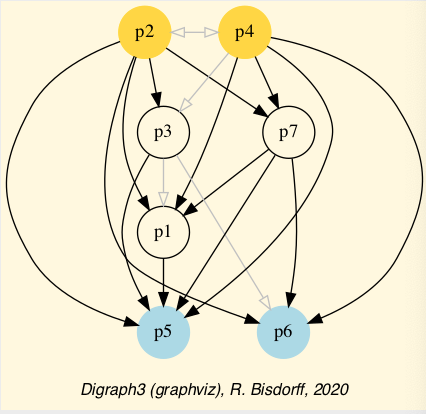
\includegraphics[height=6cm]{Figures/stdg.png}\hfill
  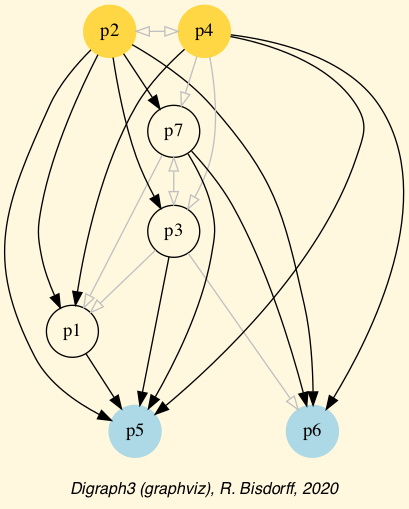
\includegraphics[height=6cm]{Figures/robg.png}
\caption{\emph{Standard} versus \emph{robust} strict outranking digraphs oriented by their initial and terminal prekernels} 
\label{fig:19.1}       % Give a unique label
\end{figure}
   
The robust version (right in Fig.~\ref{fig:19.1}) drops two strict outranking situations: between \texttt{p4} and \texttt{p7} and between \texttt{p7} and \texttt{p1}. The remaining 14 strict outranking (resp. outranked) situations are now all verified at a stability level of $+2$ and more (resp. $-2$ and less). They remain stably validated, hence, with all potential significance weights that are compatible with the given significance weights preordering (see Listing~\ref{list:19.2}).

To appreciate the apparent partial ordering of both the standard and the robust strict outranking digraphs shown in Fig.~\ref{fig:19.1}, let us have a final heat map view in Fig.~\ref{fig:19.2} on the underlying performance tableau ordered by the \NetFlows ranking rule actually applied to the robust version of the outranking digraph (see the \texttt{outrankingModel='this'} flag in Line 4 below).
\begin{lstlisting}[caption={Computing a robust performance heatmap view},label=list:19.9]
>>> rg.showHTMLPerformanceHeatmap(\
...           Correlations=True,\
...           colorLevels=5,\
...           outrankingModel='this',\
...           rankingRule='NetFlows')
\end{lstlisting}
\begin{figure}[h]
%\sidecaption
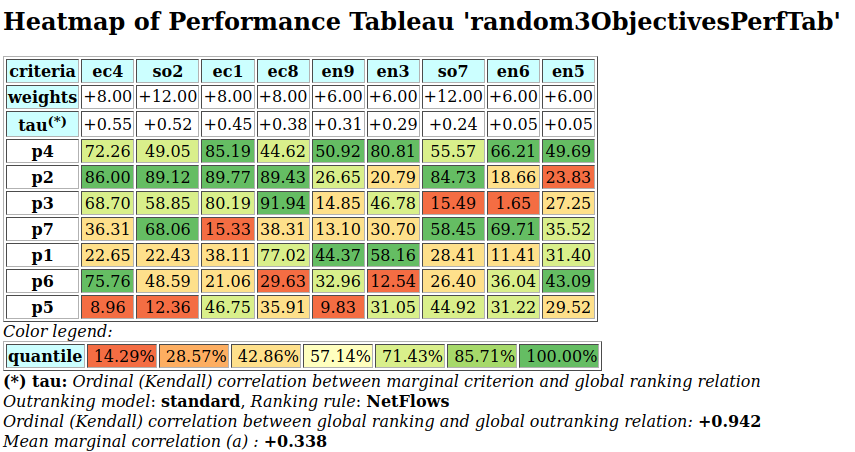
\includegraphics[width=12cm]{Figures/robustHeatmap.png}
\caption{Robust heatmap of the random 3 objectives performance tableau ordered by the \NetFlows ranking rule.} 
\label{fig:19.2}       % Give a unique label
\end{figure}
 As the inital prekernel \{\texttt{p2}, \texttt{p4}\} is in the robust outranking digraph validated at least at stability level $\pm 2$, recommending alternatives \texttt{p4}, as well as \texttt{p2}, as potential best choices, appears robustly justified. Alternative \texttt{p4} represents indeed an overall \emph{best compromise choice} between all decision objectives, whereas alternative \texttt{p2} gives an unanimous best choice with respect to two out of three decision objectives. Up to the decision maker to make his final choice.

\section{Characterising unopposed multiobjective outranking situations}
\label{sec:19.5}

When facing a performance tableau involving multiple decision objectives, the robustness level $\pm 3$  may lead to distinguishing what we call \emph{unopposed} outranking situations, like the one shown in the previous section between alternative \texttt{p4} and \texttt{p1} ($r(p4 \succsim p1) = +0.78$, see Listing \ref{list:19.4} Line 11), namely preferential situations that are more or less validated or invalidated by all the decision objectives.  
\begin{definition}[Unopposed outranking situation]\label{def:19.2}
\begin{itemize}
\item We say that decision alternative \texttt{x} \emph{unopposedly outranks} decision alternative \texttt{y} when  \texttt{x} positively outranks \texttt{y} on one or more decision objectives without \texttt{x} being positively outranked by \texttt{y} on any decision objective.
\item Dually, we say that decision alternative \texttt{x} \emph{is unopposedly outranked by} decision alternative \texttt{y} when \texttt{x} is positively outranked by \texttt{y} on one or more decision objectives without \texttt{x} positively outranking \texttt{y} on any decision objective.
\end{itemize}
\end{definition}

Let us reconsider, for instance, the performance tableau \texttt{pt} with three decision objectives already seen in Listing \ref{list:19.1}:
\begin{lstlisting}
>>> pt.showObjectives()
  *------ show objectives -------"
   Eco: Economical aspect
     ec1 criterion of objective Eco 8
     ec4 criterion of objective Eco 8
     ec8 criterion of objective Eco 8
    Total weight: 24.00 (3 criteria)
   Soc: Societal aspect
     so2 criterion of objective Soc 12
     so7 criterion of objective Soc 12
    Total weight: 24.00 (2 criteria)
   Env: Environmental aspect
     en3 criterion of objective Env 6
     en5 criterion of objective Env 6
     en6 criterion of objective Env 6
     en9 criterion of objective Env 6
    Total weight: 24.00 (4 criteria)
\end{lstlisting}
We notice in this example three decision objectives of equal importance (see Lines 3,13,17). What will be the outranking situations that are positively (resp.  negatively) validated for each one of the decision objectives taken individually ?

We may obtain such unopposed multiobjective outranking situations by operating an epistemic \emph{average fusion} (see the \texttt{symmetricAverage()} method \index{symmetricAverage@\texttt{symmetricAverage()}}) of the marginal outranking digraphs restricted to the coalition of criteria supporting each one of the decision objectives (see Listing \ref{list:19.9} below).
\begin{lstlisting}[caption={Computing unopposed outranking situations},label=list:19.9]
>>> from outrankingDigraphs import\
...                     BipolarOutrankingDigraph
>>> geco = BipolarOutrankingDigraph(pt,\
...                     objectivesSubset=['Eco'])
>>> gsoc = BipolarOutrankingDigraph(pt,\
...                     objectivesSubset=['Soc'])
>>> genv = BipolarOutrankingDigraph(pt,\
...                     objectivesSubset=['Env'])
>>> from digraphs import FusionLDigraph
>>> objectiveWeights = \
...               [pt.objectives[obj]['weight']\
...                      for obj in t.objectives] 
>>> uopg = FusionLDigraph([geco,gsoc,genv],\
...                   operator='o-average',\
...                   weights=objectiveWeights)
>>> uopg.showRelationTable(ReflexiveTerms=False)
  * ---- Relation Table -----
   r   |  'p1'   'p2'   'p3'   'p4'   'p5'   'p6'   'p7'   
  -----|------------------------------------------------
  'p1' |    -   +0.00  +0.00  -0.69  +0.39  +0.11  +0.00  
  'p2' | +0.00    -    +0.83  +0.00  +0.00  +0.00  +0.00  
  'p3' | +0.00  -0.33    -    +0.00  +0.50  +0.00  +0.00  
  'p4' | +0.78  +0.00  +0.61    -    +1.00  +1.00  +0.67  
  'p5' | -0.11  +0.00  +0.00  -0.89    -    +0.11  +0.00  
  'p6' | +0.00  +0.00  +0.00  -0.44  +0.17    -    +0.00  
  'p7' | +0.00  +0.00  +0.00  +0.00  +0.78  +0.42    -   
  Valuation domain: [-1.0; 1.0]
\end{lstlisting}
Positive (resp. negative) $r(x \succsim y)$ characteristic values, like $r(p1 \succsim p5) = +0.39$ (see Listing \ref{list:19.9} Line 20), show hence only outranking situations being validated (resp. invalidated) by one or more decision objectives without being invalidated (resp. validated) by any other decision objective.

For easily computing this kind of \emph{unopposed multiobjective} outranking digraphs, the \texttt{outrankingDigraphs} module conveniently provides a corresponding\\ \texttt{UnOpposedBipolarOutrankingDigraph} constructor \index{UnOpposedBipolarOutrankingDigraph@\texttt{UnOpposedBipolarOutrankingDigraph} class}.
\begin{lstlisting}[caption={Computing unopposed outranking digraphs},label=list:19.10]
>>> from outrankingDigraphs import\
...              UnOpposedBipolarOutrankingDigraph
>>> uopg = UnOpposedBipolarOutrankingDigraph(pt)
>>> uopg
  *------- Object instance description ------*
   Instance class      : UnOpposedBipolarOutrankingDigraph
   Instance name       : unopposed_outrankings
   Actions           : 7
   Criteria          : 9
   Size                : 13
   Oppositeness (%)    : 43.48
   Determinateness (%) : 61.71
   Valuation domain    : [-1.00;1.00]
   Attributes          : ['name', 'actions',
                'valuationdomain', 'objectives',
                'criteria', 'methodData',
                'evaluation', 'order', 'runTimes',
                'relation', ...
                'gamma', 'notGamma']
>>> uopg.computeOppositeness(InPercents=True)
  {'standardSize': 23, 'unopposedSize': 13,
   'oppositeness': 43.47826086956522}			   
\end{lstlisting}
The resulting \emph{unopposed} outranking digraph keeps in fact 13 (see Listing \ref{list:19.10} Lines 20-22) out of the 23 positively validated \emph{standard} outranking situations, leading to a degree of \emph{oppositeness} --preferential disagreement between decision objectives-- of $(1.0 - 13/23)\,=\,0.4348$.

We may now, for instance, verify the unopposed status of the outranking situation observed between alternatives \texttt{p1} and \texttt{p5}.
\begin{lstlisting}[caption={Example of unopposed multiobjective outranking situation},label=list:19.11]
>>> uopg.showPairwiseComparison('p1','p5')
 *------------  pairwise comparison ----*
  Comparing actions : ('p1', 'p5')
  crit. wght.  g(x)  g(y)    diff   | ind   pref     r()
  ec1   8.00  38.11  46.75  -8.64   | 5.00  10.00   +0.00
  ec4   8.00  22.65  8.96  +13.69   | 5.00  10.00   +8.00
  ec8   8.00  77.02  35.91  +41.11  | 5.00  10.00   +8.00
  en3   6.00  58.16  31.05  +27.11  | 5.00  10.00   +6.00
  en5   6.00  31.40  29.52  +1.88   | 5.00  10.00   +6.00
  en6   6.00  11.41  31.22  -19.81  | 5.00  10.00   -6.00
  en9   6.00  44.37  9.83  +34.54   | 5.00  10.00   +6.00
  so2   12.00  22.43  12.36  +10.07 | 5.00  10.00  +12.00
  so7   12.00  28.41  44.92  -16.51 | 5.00  10.00  -12.00
  Valuation in range: -72.00 to +72.00;           -------
                               global concordance: +28.00
\end{lstlisting}
In Listing \ref{list:19.11} we see that alternative \texttt{p1} does indeed positively outrank alternative \texttt{p5} from the economic perspective ($r(p1 \succsim_{Eco} p5) = +16/24$) as well as from the environmental perspective ($r(p1 \succsim_{Env} p5) = +12/24$). Whereas, from the societal perspective, both alternatives appear incomparable ($r(p1 \succsim_{Soc} p5) = 0/24$).

When proportionally equal criteria significance weights per objective are given, these outranking situations appear hence \emph{stable} with respect to all possible total importance weights we could allocate to the decision objectives.

This gives way for computing multiobjective \emph{Pareto efficient} choice recommendations. 

\section{Computing Pareto efficient multiobjective choices}
\label{sec:19.6}

Indeed, best choice recommendations, computed from an \emph{unopposed multiobjective} outranking digraph, deliver the case given \emph{Pareto efficient} choices. 
\begin{lstlisting}[caption={Pareto efficient multiobjective choice},label=list:19.12]
>>> uopg.showBestChoiceRecommendation()
  Best choice recommendation(s) (BCR)
   (in decreasing order of determinateness)   
   Credibility domain: [-1.00,1.00]
   === >> potential best choice(s)
   choice              : ['p2', 'p4', 'p7']
      independence        : 0.00
      dominance           : 0.33
      absorbency          : 0.00
      covering (%)        : 33.33
      determinateness (%) : 50.00
   === >> potential worst choice(s) 
   choice              : ['p3', 'p5', 'p6', 'p7']
      independence        : 0.00
      dominance           : -0.61
      absorbency          : 0.11
      covered (%)         : 33.33
      determinateness (%) : 50.00
\end{lstlisting}

Our previous \emph{robust} best choice recommendation (\texttt{p2} and \texttt{p4}, see Fig. \ref{fig:19.1}) remains, in this example here, \emph{stable}. We recover indeed the best choice recommendation [\texttt{p2}, \texttt{p4}, \texttt{p7}] (see Listing \ref{list:19.12} Line 6). Yet, notice that decision alternative \texttt{p7} appears to be at the same time a potential \emph{best} as well as a potential \emph{worst} choice recommendation (see Line 13), a consequence of \texttt{p7} being completely \emph{incomparable} to the other decision alternatives when restricting the comparability to only unopposed strict outranking situations. 

We may visualize this kind of Pareto efficient result in Fig. \ref{fig:19.3} below.
\begin{lstlisting}
>>> (~(-uopg)).exportGraphViz(fileName = 'unopDigraph',\
...                           bestChoice = ['p2','p4'],\
...                           worstChoice = ['p3','p5','p6'])
  *---- exporting a dot file for GraphViz tools ----*
   Exporting to unopDigraph.dot
   dot -Grankdir=BT -Tpng unopDigraph.dot -o unopDigraph.png
\end{lstlisting}
\begin{figure}[h]
%\sidecaption
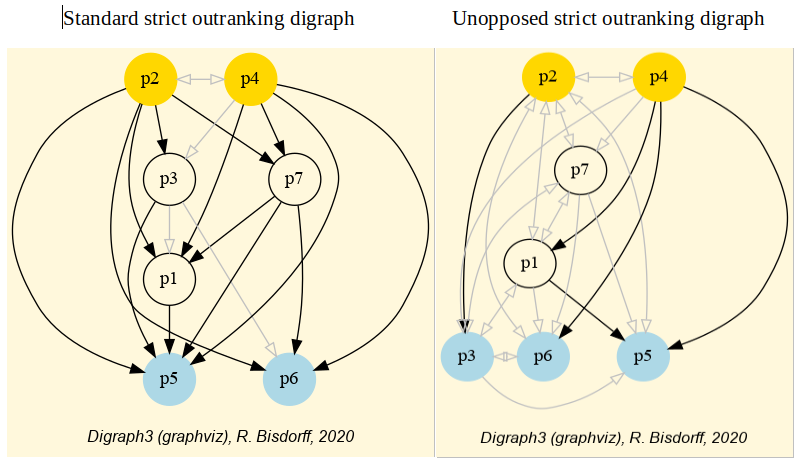
\includegraphics[width=12cm]{Figures/unopDigraph.png}
\caption{Standard versus \emph{unopposed} strict outranking digraphs oriented by best and worst choice recommendations.} 
\label{fig:19.3}       % Give a unique label
\end{figure}

In order to make now an eventual best unique choice, a decision maker will necessarily have to weight, in a second stage of the decision aiding process, the relative importance of the individual decision objectives.

\vspace{1cm}

For concluding, let us mention that it is precisely again our bipolar-valued logical characteristic framework that provides us here with a first order distributional dominance test for effectively qualifying the stability level $\pm 2$ robustness of an outranking digraph when facing performance tableaux with criteria of only ordinal-valued significances. A real world application of our stability analysis with such a kind of performance tableau may be consulted in \citep{BIS-2015}.
 
%%%%%%% The chapter bibliography
%\normallatexbib
\clearpage
%\phantomsection
%\addcontentsline{toc}{section}{Chapter Bibliography}
\bibliographystyle{spbasic}
%\typeout{}
\bibliography{03-backMatters/reference}
%\input{02-mainMatters/19-chapterRobustOutrankings.bbl}
%\bibliographystyle{spbasic}
%\bibliography{03-backMatters/reference}
